\documentclass[11pt, a4paper]{aqademic}

\usepackage[spanish]{babel}
	\selectlanguage{spanish}

\usepackage{graphicx}
  \graphicspath{{img/}}

\usepackage{pdfpages}
\usepackage{lscape}
\usepackage{hyperref}

\title{Sistema de un torneo de pádel}
\author{Expósito, Nieto, Sánchez, Requena, Romero}

\AqSetChapter{Práctica}
\AqSetSection{}

\begin{document}
\AqMaketitle[
	author    = {Javier Expósito Martínez, Inés Nieto Sánchez, Laura Sánchez Sánchez, Leire Requena Garcia, Clara María Romero Lara},
	cover      = logo-ugr.png,
	org         = Diseño y Desarrollo de Sistemas de Información
]

\tableofcontents
\chapter{Análisis y especificación de requisitos en un Sistema de Información}
	\section{Descripción del sistema}
Torneo de padel.

Se nos requiere construir un sistema para la gestión de un torneo de pádel por parejas. Este torneo se celebra en ediciones de caracter anual. El sistema administrará tanto aspectos referidos exclusivamente al juego; como cuestiones técnicas respecto a su organización. Veámoslo.


En primer lugar, los participantes del torneo. Estos compiten por parejas y, dado que no existen distintas categorías de juego dentro del sistema, cada jugador sólo puede inscribirse una vez con una única pareja.

Las parejas tienen la libertad de escoger practicar bajo la tutela de un entrenador. Cada pareja solo puede tener un entrenador asignado en un momento dado, no siendo así para los entrenadores, que pueden dirigir a cuantas parejas deseen. 

Durante el torneo, las parejas se irán posicionando en un ránking que determina sus próximos enfrentamientos.


Previa realización del torneo se abre la venta de entradas online. Para realizar un pedido se requiere una cuenta de usuario en la página web oficial. El evento se reparte en varias etapas , cada cual con su propia entrada y precio, pero existen opciones como el pase de temporada para obtener un precio reducido. Las existencias de entradas son limitadas.

Los usuarios registrados en la página pueden realizar una única compra al día, y solo una compra puede estar activa en carrito. Cuando finaliza una compra, se les envía un recibo con toda la información pertinente; este se puede imprimir en casa, mostrar desde el teléfono móvil, o decir en taquilla el número identificador único a cada entrada.


Las contratas de los árbitros también se gestionan desde el sistema. Funciona bajo un sistema de mejor postor, en el que los árbitros reciben múltiples ofertas, que pueden aceptar, rechazar o contraofertar. 

El intercambio de ofertas entre postor y árbitro funciona tal que una oferta puede ser o bien aceptada o rechazada, acabando ahí; o bien ser contraofertada. El postor inicial es ahora quién se responsabiliza de aceptar o denegar esta contraoferta. Ahí termina el ciclo de vida de la oferta inicial: si el postor no está de acuerdo con la contraoferta recibida, se debe iniciar un proceso de oferta nuevo. 

Una vez cualquiera de las dos partes han aceptado o rechazado una oferta o contraoferta, la decisión es definitiva, y la oferta no puede ser modificada de ninguna manera.


Dentro de lo que es el torneo, existe una asignación de partidos a las pistas del recinto. Los partidos se juegan con un árbitro preasignado que, obviamente, ha aceptado una oferta para trabajar en el susodicho. Sin embargo, un árbitro solo puede pitar un partido diario.

Los partidos se asignan de forma previa a las pistas para poder publicar un horario con las correspondencias del día. La jornada del torneo dura 8 horas, y tras cada partido debe haber un periodo mínimo de 3 horas para la correcta limpieza y preparación de la pista y gradas. Por esto, en un mismo día no puede haber más de dos partidos en una misma pista.

Los resultados de los partidos se registrarán y harán públicos tras su finalización, con objeto de emplear estos datos en la elaboración del ránking.


El personal del evento se organizará por turnos delimitados en el día según horario y pista. Los turnos de un trabajador no deben solaparse con menos de una hora de diferencia para darle tiempo para abandonar el turno en la pista previa y llegar a la siguiente, además de un breve descanso. Un empleado no trabajará más de 8 horas en un día, y puede trabajar como máximo dos veces la misma pista en el día.

Una vez un empleado ha fichado para el día, no se puede modificar su salario previamente acordado.


Este evento cuenta con la colaboración y patrocinio de entidades externas a la organización. Este puede ser monetario o de material, y cuando una entidad se registra como patrocinador o colaborador, no se puede modificar durante la edición. Una vez el torneo ha comenzado, tampoco se les permite retirarse o modificar la cantidad monetaria aportada.


Finalmente, el material necesario para el torneo se suministra por pedidos por correo. Estos pedidos deben de ser recogidos por un empleado de la organización para firmar el albarán: todos los pedidos deben ser confirmados al llegar, y se recogen en una de las pistas del polideportivo. 

Los trabajadores de la pista durante el horario de llegada son los encargados de recibirlo, pero se debe notificar al trabajador con mínimo una hora de antelación. La asignación no es revocable: bajo ningún concepto se permite la cancelación de un pedido ya asignado a un trabajador.

Los pedidos son provistos por los patrocinadores, así que cada pedido corresponde únicamente a una entidad patrocinadora.


Estas son todas las características e indicaciones relevantes a este sistema de torneos de pádel. A continuación serán desglosadas en forma de requisitos y restricciones




	\pagebreak
	\section{Reparto de los subsistemas}
\subsection{Jugadores-Entrenadores: Clara María Romero Lara}
\subsubsection{Requisitos funcionales}
\begin{itemize}
	\item Insertar nuevo jugador en la base de datos
	\item Asignar entrenador a pareja en una edición del torneo
	\item Consultar entrenadores y parejas que entrena en esa edición
	\item Inscribir pareja de jugadores en una edición
	\item Mostrar las parejas de jugadores por ranking en una edición
\end{itemize}

\subsubsection{Condiciones}
\begin{itemize}
	\item Una pareja sólo puede tener un entrenador en una edición
	\item Un jugador no puede pertenecer a dos parejas distintas en la misma edición
\end{itemize}

\subsection{Pistas-Partidos: Javier Expósito Martínez}
\subsubsection{Requisitos funcionales}
\begin{itemize}
	\item Insertar partido
	\item Añadir resultado a un partido
	\item Mostrar los partidos que se juegan en una pista en una edición
	\item Cambiar el árbitro de un partido
	\item Mostrar pistas sin ningún partido asignado en esa edición
\end{itemize}

\subsubsection{Condiciones}
\begin{itemize}
	\item No se pueden solapar los horarios de dos partidos en una misma pista con menos de 3 horas de diferencia
	\item En una misma pista no se pueden jugar más de dos partidos en el mismo día
	\item Sólo puedo asignar árbitros que hayan aceptado una oferta en esta edición
	\item Un árbitro no puede llevar más de un partido por día
	\item No se puede añadir un resultado a un partido cuya fecha de inicio es posterior a la fecha actual
\end{itemize}

\subsection{Patrocinadores-Colaboradores: Leire Requena Garcia}
\subsubsection{Requisitos funcionales}
\begin{itemize}
	\item Insertar una nueva entidad
	\item Registrar entidad como colaborador en una edición
	\item Mostrar dinero total obtenido en una edición
	\item Modificar el dinero aportado por un colaborador en una edición
	\item Eliminar patrocinador de una edición
\end{itemize}

\subsubsection{Condiciones}
\begin{itemize}
	\item Una entidad no puede colaborar y patrocinar en la misma edición
	\item No se puede modificar el dinero aportado por un colaborador o patrocinador si ya ha comenzado el torneo
	\item No se puede eliminar un patrocinador o colaborador si ya ha comenzado el torneo
\end{itemize}

\subsection{Personal-Horarios: Laura Sánchez Sánchez}
\subsubsection{Requisitos funcionales}
\begin{itemize}
	\item Trabajar en una edición.
	\item Asignar horario de trabajo a un trabajador.
	\item Mostrar el personal que no trabaja en una edición.
	\item Mostrar el total de salarios pagados en una edición.
	\item Mostrar los trabajadores de una edición ordenados por horas trabajadas.
\end{itemize}

\subsubsection{Condiciones}
\begin{itemize}
	\item No se pueden solapar los horarios de un trabajador con menos de una hora de diferencia
	\item No se puede asignar a un trabajador la misma pista más de dos veces el mismo día
	\item No se puede trabajar más de 8 horas el mismo día
	\item No puedo modificar el salario de un trabajador si ya ha realizado algún trabajo
\end{itemize}

\subsection{Materiales-Pedidos: Inés Nieto Sánchez}
\subsubsection{Requisitos funcionales}
\begin{itemize}
	\item Insertar nuevo material en una edición.
	\item Realizar pedido de materiales en una edición.
	\item Asignar pedido a un trabajador.
	\item Cancelar la asignación de un pedido.
	\item Mostrar pedidos realizados por un patrocinador en una edición.
\end{itemize}

\subsubsection{Condiciones}
\begin{itemize}
	\item Un pedido sólo puede contener materiales del mismo patrocinador
	\item No puedo asignar un pedido a un trabajador que no está trabajando a esa hora en esa pista
	\item No se puede cancelar un pedido que ya esté asignado a un trabajador
	\item No puedo cancelar la asignación de un pedido a un trabajador el mismo día en el que se va a entregar
	\item No puedo asignar un nuevo pedido al mismo trabajador con menos de una hora de diferencia
	\item Sólo se puede marcar un pedido como recibido después de la fecha en la que estaba prevista la entrega
\end{itemize}


	\pagebreak
	\section{Especificación de los requisitos funcionales}

\subsection{Jugadores-Entrenadores}

\subsubsection{RF1.1: Insertar nuevo jugador en la base de datos}

\textbf{Entrada:} Agente externo: Jugador        Requisito de datos de entrada: RDE1.1

\textbf{BD:} Requisito de datos de escritura RDW1.1

\textbf{Salida:} Agente externo: ninguno

Requisito de datos de salida: ninguno

\textbf{RDE1.1:} Datos de entrada de jugador:
\begin{itemize}
	\item Nombre: cadena de caracteres (30)
	\item Apellidos: cadena de caracteres (60)
	\item Teléfono: cadena numérica (12, el primero puede ser +)
	\item E-mail: cadena de caracteres (50, debe contener @)
\end{itemize}
\textbf{RDW1.1:} Datos almacenados del jugador:
\begin{itemize}
	\item Nombre: cadena de caracteres (30)
	\item Apellidos: cadena de caracteres (60)
	\item Teléfono: cadena numérica (12, el primero puede ser +)
	\item E-mail: cadena de caracteres (50, debe contener @)
\end{itemize}


\subsubsection{RF1.2: Asignar entrenador a pareja en una edición del torneo}

\textbf{Entrada:} Agente externo: Jugador        Requisito de datos de entrada: RDE1.2

\textbf{BD:} Requisito de datos de escritura RDW1.2, requisito de datos de lectura RDR1.1

\textbf{Salida:} Agente externo: ninguno

Requisito de datos de salida: ninguno

\textbf{RDE1.2:} Datos de entrada de entrenador, la pareja y la edición:
\begin{itemize}
	\item Edición: número entero (4, corresponde al año)
\newline
	\item Nombre jugador 1: cadena de caracteres (30)
	\item Apellidos jugador 1: cadena de caracteres (60)
	\item Teléfono jugador 1: cadena numérica (12, el primero puede ser +)
	\item E-mail jugador 1l: cadena de caracteres (50, debe contener la @)
\newline
	\item Nombre jugador 2: cadena de caracteres (30)
	\item Apellidos jugador 2: cadena de caracteres (60)
	\item Teléfono jugador 2: cadena numérica (12, el primero puede ser +)
	\item E-mail jugador 2: cadena de caracteres (50)
\newline
	\item Nombre entrenador: cadena de caracteres (30)
	\item Apellidos entrenador: cadena de caracteres (60)
	\item Teléfono entrenador: cadena numérica (12, el primero puede ser +)
	\item E-mail entrenador: cadena de caracteres (50)
\end{itemize}

\textbf{RDW1.2:} Datos almacenados de la pareja:
\begin{itemize}
	\item Nombre jugador 1: cadena de caracteres (30)
	\item Apellidos jugador 1: cadena de caracteres (60)
	\item Teléfono jugador 1: cadena numérica (12, el primero puede ser +)
	\item E-mail jugador 1: cadena de caracteres (50, debe contener la @)
\newline
	\item Nombre jugador 2: cadena de caracteres (30)
	\item Apellidos jugador 2: cadena de caracteres (60)
	\item Teléfono jugador 2: cadena numérica (12, el primero puede ser  +)
	\item E-mail jugador 2: cadena de caracteres (50)
\newline
	\item Nombre entrenador: cadena de caracteres (30)
	\item Apellidos entrenador: cadena de caracteres (60)
	\item Teléfono entrenador: cadena numérica (12, el primero puede ser +)
	\item E-mail entrenador: cadena de caracteres (50)
\end{itemize}

\textbf{RDR1.1:} Datos de salida de la pareja:
\begin{itemize}
	\item Nombre jugador 1: cadena de caracteres (30)
	\item Apellidos jugador 1: cadena de caracteres (60)
	\item Teléfono jugador 1: cadena numérica (12, el primero puede ser +)
	\item E-mail jugador 1: cadena de caracteres (50, debe contener la @)
\newline
	\item Nombre jugador 2: cadena de caracteres (30)
	\item Apellidos jugador 2: cadena de caracteres (60)
	\item Teléfono jugador 2: cadena numérica (12, el primero puede ser  +)
	\item E-mail jugador 2: cadena de caracteres (50)
\newline
	\item Nombre entrenador: cadena de caracteres (30)
	\item Apellidos entrenador: cadena de caracteres (60)
	\item Teléfono entrenador: cadena numérica (12, el primero puede ser +)
	\item E-mail entrenador: cadena de caracteres (50)
\end{itemize}

\subsubsection{RF1.3: Consultar entrenadores y parejas que entrena en esa edición}

\textbf{Entrada:} Agente externo: Organizador    Requisito de datos de entrada: RDE1.3

\textbf{BD:} Requisito de datos de lectura RDR1.2

\textbf{Salida:} Agente externo: Organizador

Requisito de datos de salida: RDS1.1

\textbf{RDE1.3:} Datos de entrada de edición:
\begin{itemize}
	\item Edición: número entero (4, corresponde al año)
\end{itemize}

\textbf{RDR1.2:} Datos de lectura de pareja y entrenador:
\begin{itemize}
	\item Edición: número entero (4 cifras)
\newline
	\item Nombre jugador 1: cadena de caracteres (30)
	\item Apellidos jugador 1: cadena de caracteres (60)
	\item Teléfono jugador 1: cadena numérica (12, el primero puede ser +)
	\item E-mail jugador 1: cadena de caracteres (50, debe contener la @)
\newline
	\item Nombre jugador 2: cadena de caracteres (30)
	\item Apellidos jugador 2: cadena de caracteres (60)
	\item Teléfono jugador 2: cadena numérica (12, el primero puede ser  +)
	\item E-mail jugador 2: cadena de caracteres (50)
\newline
	\item Nombre entrenador: cadena de caracteres (30)
	\item Apellidos entrenador: cadena de caracteres (60)
	\item Teléfono entrenador: cadena numérica (12, el primero puede ser  +)
	\item E-mail entrenador: cadena de caracteres (50, debe contener la @)
\end{itemize}

\textbf{RDS1.1:} Datos de salida de pareja y entrenador:
\begin{itemize}
	\item Nombre jugador 1: cadena de caracteres (30)
	\item Apellidos jugador 1: cadena de caracteres (60)
	\item Teléfono jugador 1: cadena numérica (12, el primero puede ser +)
	\item E-mail jugador 1: cadena de caracteres (50, debe contener la @)
\newline
	\item Nombre jugador 2: cadena de caracteres (30)
	\item Apellidos jugador 2: cadena de caracteres (60)
	\item Teléfono jugador 2: cadena numérica (12, el primero puede ser  +)
	\item E-mail jugador 2: cadena de caracteres (50)
\end{itemize}

\subsubsection{RF1.4: Inscribir pareja de jugadores en una edición}

\textbf{Entrada:} Agente externo: Jugador        Requisito de datos de entrada: RDE1.4

\textbf{BD:} Requisito de datos de escritura RDW1.3, requisito de datos de lectura RDR1.3

\textbf{Salida:} Agente externo: ninguno

Requisito de datos de salida: ninguno

\textbf{RDE1.4:} Datos de entrada de la pareja:
\begin{itemize}
	\item Edición: número entero (4, corresponde al año)
\newline
	\item Nombre jugador 1: cadena de caracteres (30)
	\item Apellidos jugador 1: cadena de caracteres (60)
	\item Teléfono jugador 1: cadena numérica (12, el primero puede ser +)
	\item E-mail jugador 1: cadena de caracteres (50, debe contener la @)
\newline
	\item Nombre jugador 2: cadena de caracteres (30)
	\item Apellidos jugador 2: cadena de caracteres (60)
	\item Teléfono jugador 2: cadena numérica (12, el primero puede ser  +)
	\item E-mail jugador 2: cadena de caracteres (50)
\end{itemize}

\textbf{RDW1.3:} Datos almacenados del jugador:
\begin{itemize}
	\item Edición: número entero (4 cifras)
\newline
	\item Nombre jugador 1: cadena de caracteres (30)
	\item Apellidos jugador 1: cadena de caracteres (60)
	\item Teléfono jugador 1: cadena numérica (12, el primero puede ser +)
	\item E-mail jugador 1: cadena de caracteres (50, debe contener la @)
\newline
	\item Nombre jugador 2: cadena de caracteres (30)
	\item Apellidos jugador 2: cadena de caracteres (60)
	\item Teléfono jugador 2: cadena numérica (12, el primero puede ser  +)
	\item E-mail jugador 2: cadena de caracteres (50)
\end{itemize}

\textbf{RDR1.3:} Datos de salida del jugador:
\begin{itemize}
	\item Edición: número entero (4 cifras)
\newline
	\item Nombre jugador 1: cadena de caracteres (30)
	\item Apellidos jugador 1: cadena de caracteres (60)
	\item Teléfono jugador 1: cadena numérica (12, el primero puede ser +)
	\item E-mail jugador 1: cadena de caracteres (50, debe contener la @)
\newline
	\item Nombre jugador 2: cadena de caracteres (30)
	\item Apellidos jugador 2: cadena de caracteres (60)
	\item Teléfono jugador 2: cadena numérica (12, el primero puede ser  +)
	\item E-mail jugador 2: cadena de caracteres (50)
\end{itemize}


\subsubsection{RF1.5: Mostrar las parejas de jugadores por ranking en una edición}

\textbf{Entrada:} Agente externo: Organizador        Requisito de datos de entrada: RDE1.5

\textbf{BD:} Requisito de datos de lectura RDR1.4

\textbf{Salida:} Agente externo: Organizador

Requisito de datos de salida: RDS1.2

\textbf{RDE1.5:} Datos de entrada de ranking y edición:
\begin{itemize}
	\item Edición: número entero (4, corresponde al año)
	\item Cota superior: número entero
\end{itemize}

\textbf{RDR1.1:} Datos almacenados del jugador:
\begin{itemize}
	\item Edición: número entero (4 cifras)
	\item Posición ranking: número entero (hasta 2 cifras)
\newline
	\item Nombre jugador 1: cadena de caracteres (30)
	\item Apellidos jugador 1: cadena de caracteres (60)
	\item Teléfono jugador 1: cadena numérica (12, el primero puede ser +)
	\item E-mail jugador 1: cadena de caracteres (50, debe contener la @)
\newline
	\item Nombre jugador 2: cadena de caracteres (30)
	\item Apellidos jugador 2: cadena de caracteres (60)
	\item Teléfono jugador 2: cadena numérica (12, el primero puede ser  +)
	\item E-mail jugador 2: cadena de caracteres (50)
\end{itemize}

\textbf{RDS1.2:} Datos almacenados del jugador:
\begin{itemize}
	\item Posición de la pareja: número entero (hasta 2 cifras)
\newline
	\item Nombre jugador 1: cadena de caracteres (30)
	\item Apellidos jugador 1: cadena de caracteres (60)
	\item Teléfono jugador 1: cadena numérica (12, el primero puede ser +)
	\item E-mail jugador 1: cadena de caracteres (50, debe contener la @)
\newline
	\item Nombre jugador 2: cadena de caracteres (30)
	\item Apellidos jugador 2: cadena de caracteres (60)
	\item Teléfono jugador 2: cadena numérica (12, el primero puede ser  +)
	\item E-mail jugador 2: cadena de caracteres (50)
\end{itemize}

\subsubsection{RS1.1: Una pareja solo puede tener un entrenador en una edición}
\textbf{RF:} RF1.2

\textbf{RD(s):} RDE1.2,RDR1.1

\textbf{Descripción:} Si ya existe un entrenador asignado a la pareja, el nuevo entrenador no se registra y se da un mensaje de error

\subsubsection{RS1.2: Un jugador no puede pertenecer a dos parejas distintas en la misma edición}
\textbf{RF:} RF1.4

\textbf{RD(s):} RDE1.4, RDR1.3

\textbf{Descripción:} Si un jugador que ya pertenece a una pareja se intenta registrar con otra, la nueva pareja no se registra y se da un mensaje de error
\pagebreak


\subsection{Pistas-Partidos}

\subsubsection{RF2.1: Insertar partido}
\textbf{Entrada:} Agente externo: Organizador    Requisito de datos de entrada:RDE2.1

\textbf{BD:} Requisito de datos de  escritura RDW2.1, requisito de datos de lectura RDR2.1

\textbf{Salida:} Agente externo:Ninguno

Requisito de datos de salida:

\textbf{RDE2.1:} Datos de entrada del partido
\begin{itemize}
	\item Edición: Número entero de 4 cifras
\newline
	\item Nombre jugador 1: cadena de caracteres (30)
	\item Apellidos jugador 1: cadena de caracteres (60)
	\item Teléfono jugador 1: cadena numérica (12, el primero puede ser +)
	\item E-mail jugador 1: cadena de caracteres (50, debe contener @)
\newline
	\item Nombre jugador 2: cadena de caracteres (30)
	\item Apellidos jugador 2: cadena de caracteres (60)
	\item Teléfono jugador 2: cadena numérica (12, el primero puede ser +)
	\item E-mail jugador 2: cadena de caracteres (50, debe contener @)
\newline
	\item Nombre jugador 3: cadena de caracteres (30)
	\item Apellidos jugador 3: cadena de caracteres (60)
	\item Teléfono jugador 3: cadena numérica (12, el primero puede ser +)
	\item E-mail jugador 3: cadena de caracteres (50, debe contener @)
\newline
	\item Nombre jugador 4: cadena de caracteres (30)
	\item Apellidos jugador 4: cadena de caracteres (60)
	\item Teléfono jugador 4: cadena numérica (12, el primero puede ser +)
	\item E-mail jugador 4: cadena de caracteres (50, debe contener @)
\newline
	\item Nombre árbitro: cadena de caracteres (30)
	\item Apellidos árbitro: cadena de caracteres (60)
	\item Teléfono árbitro: cadena numérica (12, el primero puede ser +)
	\item E-mail árbitro: cadena de caracteres (50, debe contener @)
\newline
	\item Nombre pista: cadena de caracteres (30)
	\item Capacidad pista : número entero (4 cifras)
	\item Fecha: cadena numérica (DD-MM-AAAA HH:MM:SS)

\end{itemize}

\textbf{RDW2.1:} Datos almacenados del partido
\begin{itemize}
	\item Edición: Número entero de 4 cifras
\newline
	\item Nombre jugador 1: cadena de caracteres (30)
	\item Apellidos jugador 1: cadena de caracteres (60)
	\item Teléfono jugador 1: cadena numérica (12, el primero puede ser +)
	\item E-mail jugador 1: cadena de caracteres (50, debe contener @)
\newline
	\item Nombre jugador 2: cadena de caracteres (30)
	\item Apellidos jugador 2: cadena de caracteres (60)
	\item Teléfono jugador 2: cadena numérica (12, el primero puede ser +)
	\item E-mail jugador 2: cadena de caracteres (50, debe contener @)
\newline
	\item Nombre jugador 3: cadena de caracteres (30)
	\item Apellidos jugador 3: cadena de caracteres (60)
	\item Teléfono jugador 3: cadena numérica (12, el primero puede ser +)
	\item E-mail jugador 3: cadena de caracteres (50, debe contener @)
\newline
	\item Nombre jugador 4: cadena de caracteres (30)
	\item Apellidos jugador 4: cadena de caracteres (60)
	\item Teléfono jugador 4: cadena numérica (12, el primero puede ser +)
	\item E-mail jugador 4: cadena de caracteres (50, debe contener @)
\newline
	\item Nombre árbitro: cadena de caracteres (30)
	\item Apellidos árbitro: cadena de caracteres (60)
	\item Teléfono árbitro: cadena numérica (12, el primero puede ser +)
	\item E-mail árbitro: cadena de caracteres (50, debe contener @)
\newline
	\item Nombre pista: cadena de caracteres (30)
	\item Capacidad pista : número entero (4 cifras)
	\item Fecha: cadena numérica (DD-MM-AAAA HH:MM:SS)
\end{itemize}

\textbf{RDR2.1:} Datos de lectura de la pista en la que se jugará el partido
\begin{itemize}
	\item Nombre pista: cadena de caracteres (30)
	\item Capacidad pista : número entero (4 cifras)
	\item Fecha: cadena numérica (DD-MM-AAAA HH:MM:SS)
\end{itemize}

\subsubsection{RF2.2: Añadir resultado a un partido}
\textbf{Entrada:} Agente externo:Organizador    Requisito de datos de entrada: RDE2.2

\textbf{BD:} Requisito de datos de  escritura RDW2.2, requisito de datos de lectura RDR2.2

\textbf{Salida:} Ninguna   Agente externo: Ninguno

Requisito de datos de salida:

\textbf{RDE2.2:} Datos de entrada del resultado
\begin{itemize}
	\item Edición: Número entero de 4 cifras
\newline
	\item Nombre jugador 1: cadena de caracteres (30)
	\item Apellidos jugador 1: cadena de caracteres (60)
	\item Teléfono jugador 1: cadena numérica (12, el primero puede ser +)
	\item E-mail jugador 1: cadena de caracteres (50, debe contener @)
\newline
	\item Nombre jugador 2: cadena de caracteres (30)
	\item Apellidos jugador 2: cadena de caracteres (60)
	\item Teléfono jugador 2: cadena numérica (12, el primero puede ser +)
	\item E-mail jugador 2: cadena de caracteres (50, debe contener @)
\newline
	\item Nombre jugador 3: cadena de caracteres (30)
	\item Apellidos jugador 3: cadena de caracteres (60)
	\item Teléfono jugador 3: cadena numérica (12, el primero puede ser +)
	\item E-mail jugador 3: cadena de caracteres (50, debe contener @)
\newline
	\item Nombre jugador 4: cadena de caracteres (30)
	\item Apellidos jugador 4: cadena de caracteres (60)
	\item Teléfono jugador 4: cadena numérica (12, el primero puede ser +)
	\item E-mail jugador 4: cadena de caracteres (50, debe contener @)
\newline
	\item Nombre árbitro: cadena de caracteres (30)
	\item Apellidos árbitro: cadena de caracteres (60)
	\item Teléfono árbitro: cadena numérica (12, el primero puede ser +)
	\item E-mail árbitro: cadena de caracteres (50, debe contener @)
\newline
	\item Nombre pista: cadena de caracteres (30)
	\item Capacidad pista : número entero (4 cifras)
	\item Fecha: cadena numérica (DD-MM-AAAA HH:MM:SS)
\newline
	\item Nº sets pareja 1: número entero (1 cifras)
	\item Nº sets pareja 2: número entero (1 cifras)
\end{itemize}


\textbf{RDW2.2:} Datos almacenados del resultado
\begin{itemize}
	\item Edición: Número entero de 4 cifras
\newline
	\item Nombre jugador 1: cadena de caracteres (30)
	\item Apellidos jugador 1: cadena de caracteres (60)
	\item Teléfono jugador 1: cadena numérica (12, el primero puede ser +)
	\item E-mail jugador 1: cadena de caracteres (50, debe contener @)
\newline
	\item Nombre jugador 2: cadena de caracteres (30)
	\item Apellidos jugador 2: cadena de caracteres (60)
	\item Teléfono jugador 2: cadena numérica (12, el primero puede ser +)
	\item E-mail jugador 2: cadena de caracteres (50, debe contener @)
\newline
	\item Nombre jugador 3: cadena de caracteres (30)
	\item Apellidos jugador 3: cadena de caracteres (60)
	\item Teléfono jugador 3: cadena numérica (12, el primero puede ser +)
	\item E-mail jugador 3: cadena de caracteres (50, debe contener @)
\newline
	\item Nombre jugador 4: cadena de caracteres (30)
	\item Apellidos jugador 4: cadena de caracteres (60)
	\item Teléfono jugador 4: cadena numérica (12, el primero puede ser +)
	\item E-mail jugador 4: cadena de caracteres (50, debe contener @)
\newline
	\item Nombre árbitro: cadena de caracteres (30)
	\item Apellidos árbitro: cadena de caracteres (60)
	\item Teléfono árbitro: cadena numérica (12, el primero puede ser +)
	\item E-mail árbitro: cadena de caracteres (50, debe contener @)
\newline
	\item Nombre pista: cadena de caracteres (30)
	\item Capacidad pista : número entero (4 cifras)
	\item Fecha: cadena numérica (DD-MM-AAAA HH:MM:SS)
\newline
	\item Resultado: cadena de caracteres(30)
	\item Nº sets pareja 1: número entero (1 cifras)
	\item Nº sets pareja 2: número entero (1 cifras)
\end{itemize}

\textbf{RDR2.2: }Fecha en la que se juega el partido
\begin{itemize}
	\item Fecha: cadena numérica (DD-MM-AAAA HH:MM:SS)
\end{itemize}
     
\subsubsection{RF2.3: Mostrar partidos que se juegan en una pista en una edición}
\textbf{Entrada:} Agente externo: Organizador        Requisito de datos de entrada: RDE2.3

\textbf{BD:} Requisito de datos de  lectura RDR2.3

\textbf{Salida:} Agente externo:Organizador

Requisito de datos de salida: RDS2.1

\textbf{RDE2.3:} Datos de entrada para la búsqueda de los partidos
\begin{itemize}
	\item Edición: número entero de 4 cifras
	\item Nombre de la pista: cadena de caracteres (30)
	\item Capacidad pista : número entero (4 cifras)
\end{itemize}

\textbf{RDR2.3:} Datos de lectura de los partidos
\begin{itemize}
	\item Edición: Número entero de 4 cifras
\newline
	\item Nombre jugador 1: cadena de caracteres (30)
	\item Apellidos jugador 1: cadena de caracteres (60)
	\item Teléfono jugador 1: cadena numérica (12, el primero puede ser +)
	\item E-mail jugador 1: cadena de caracteres (50, debe contener @)
\newline
	\item Nombre jugador 2: cadena de caracteres (30)
	\item Apellidos jugador 2: cadena de caracteres (60)
	\item Teléfono jugador 2: cadena numérica (12, el primero puede ser +)
	\item E-mail jugador 2: cadena de caracteres (50, debe contener @)
\newline
	\item Nombre jugador 3: cadena de caracteres (30)
	\item Apellidos jugador 3: cadena de caracteres (60)
	\item Teléfono jugador 3: cadena numérica (12, el primero puede ser +)
	\item E-mail jugador 3: cadena de caracteres (50, debe contener @)
\newline
	\item Nombre jugador 4: cadena de caracteres (30)
	\item Apellidos jugador 4: cadena de caracteres (60)
	\item Teléfono jugador 4: cadena numérica (12, el primero puede ser +)
	\item E-mail jugador 4: cadena de caracteres (50, debe contener @)
\newline
	\item Nombre árbitro: cadena de caracteres (30)
	\item Apellidos árbitro: cadena de caracteres (60)
	\item Teléfono árbitro: cadena numérica (12, el primero puede ser +)
	\item E-mail árbitro: cadena de caracteres (50, debe contener @)
\newline
	\item Nombre pista: cadena de caracteres (30)
	\item Capacidad pista : número entero (4 cifras)
	\item Fecha: cadena numérica (DD-MM-AAAA HH:MM:SS)
\end{itemize}

\textbf{RDS2.1:} Datos de salida de los partidos
\begin{itemize}
	\item Edición: Número entero de 4 cifras
\newline
	\item Nombre jugador 1: cadena de caracteres (30)
	\item Apellidos jugador 1: cadena de caracteres (60)
	\item Teléfono jugador 1: cadena numérica (12, el primero puede ser +)
	\item E-mail jugador 1: cadena de caracteres (50, debe contener @)
\newline
	\item Nombre jugador 2: cadena de caracteres (30)
	\item Apellidos jugador 2: cadena de caracteres (60)
	\item Teléfono jugador 2: cadena numérica (12, el primero puede ser +)
	\item E-mail jugador 2: cadena de caracteres (50, debe contener @)
\newline
	\item Nombre jugador 3: cadena de caracteres (30)
	\item Apellidos jugador 3: cadena de caracteres (60)
	\item Teléfono jugador 3: cadena numérica (12, el primero puede ser +)
	\item E-mail jugador 3: cadena de caracteres (50, debe contener @)
\newline
	\item Nombre jugador 4: cadena de caracteres (30)
	\item Apellidos jugador 4: cadena de caracteres (60)
	\item Teléfono jugador 4: cadena numérica (12, el primero puede ser +)
	\item E-mail jugador 4: cadena de caracteres (50, debe contener @)
\newline
	\item Nombre árbitro: cadena de caracteres (30)
	\item Apellidos árbitro: cadena de caracteres (60)
	\item Teléfono árbitro: cadena numérica (12, el primero puede ser +)
	\item E-mail árbitro: cadena de caracteres (50, debe contener @)
\newline
	\item Nombre pista: cadena de caracteres (30)
	\item Capacidad pista : número entero (4 cifras)
	\item Fecha: cadena numérica (DD-MM-AAAA HH:MM:SS)
\end{itemize}

\subsubsection{RF2.4: Cambiar árbitro de un partido}
\textbf{Entrada:} Agente externo: Organizador        Requisito de datos de entrada: RDE2.4

\textbf{BD:} Requisito de datos de  escritura RDW2.3

\textbf{Salida:} Agente externo:

Requisito de datos de salida: Ninguno

\textbf{RDE2.4:} Datos de entrada del árbitro nuevo
\begin{itemize}
	\item Edición: Número entero de 4 cifras
\newline
	\item Nombre jugador 1: cadena de caracteres (30)
	\item Apellidos jugador 1: cadena de caracteres (60)
	\item Teléfono jugador 1: cadena numérica (12, el primero puede ser +)
	\item E-mail jugador 1: cadena de caracteres (50, debe contener @)
\newline
	\item Nombre jugador 2: cadena de caracteres (30)
	\item Apellidos jugador 2: cadena de caracteres (60)
	\item Teléfono jugador 2: cadena numérica (12, el primero puede ser +)
	\item E-mail jugador 2: cadena de caracteres (50, debe contener @)
\newline
	\item Nombre jugador 3: cadena de caracteres (30)
	\item Apellidos jugador 3: cadena de caracteres (60)
	\item Teléfono jugador 3: cadena numérica (12, el primero puede ser +)
	\item E-mail jugador 3: cadena de caracteres (50, debe contener @)
\newline
	\item Nombre jugador 4: cadena de caracteres (30)
	\item Apellidos jugador 4: cadena de caracteres (60)
	\item Teléfono jugador 4: cadena numérica (12, el primero puede ser +)
	\item E-mail jugador 4: cadena de caracteres (50, debe contener @)
\newline
	\item Nombre árbitro: cadena de caracteres (30)
	\item Apellidos árbitro: cadena de caracteres (60)
	\item Teléfono árbitro: cadena numérica (12, el primero puede ser +)
	\item E-mail árbitro: cadena de caracteres (50, debe contener @)
\newline
	\item Nombre pista: cadena de caracteres (30)
	\item Capacidad pista : número entero (4 cifras)
	\item Fecha: cadena numérica (DD-MM-AAAA HH:MM:SS)
\end{itemize}

\textbf{RDW2.3:} Datos de escritura del árbitro nuevo
\begin{itemize}
	\item Edición: Número entero de 4 cifras
\newline
	\item Nombre jugador 1: cadena de caracteres (30)
	\item Apellidos jugador 1: cadena de caracteres (60)
	\item Teléfono jugador 1: cadena numérica (12, el primero puede ser +)
	\item E-mail jugador 1: cadena de caracteres (50, debe contener @)
\newline
	\item Nombre jugador 2: cadena de caracteres (30)
	\item Apellidos jugador 2: cadena de caracteres (60)
	\item Teléfono jugador 2: cadena numérica (12, el primero puede ser +)
	\item E-mail jugador 2: cadena de caracteres (50, debe contener @)
\newline
	\item Nombre jugador 3: cadena de caracteres (30)
	\item Apellidos jugador 3: cadena de caracteres (60)
	\item Teléfono jugador 3: cadena numérica (12, el primero puede ser +)
	\item E-mail jugador 3: cadena de caracteres (50, debe contener @)
\newline
	\item Nombre jugador 4: cadena de caracteres (30)
	\item Apellidos jugador 4: cadena de caracteres (60)
	\item Teléfono jugador 4: cadena numérica (12, el primero puede ser +)
	\item E-mail jugador 4: cadena de caracteres (50, debe contener @)
\newline
	\item Nombre árbitro: cadena de caracteres (30)
	\item Apellidos árbitro: cadena de caracteres (60)
	\item Teléfono árbitro: cadena numérica (12, el primero puede ser +)
	\item E-mail árbitro: cadena de caracteres (50, debe contener @)
\newline
	\item Nombre pista: cadena de caracteres (30)
	\item Capacidad pista : número entero (4 cifras)
	\item Fecha: cadena numérica (DD-MM-AAAA HH:MM:SS)
\end{itemize}

\subsubsection{RF2.5:Mostrar pistas sin ningún partido asignado en esta edición}
\textbf{Entrada:} Agente externo: Organizador        Requisito de datos de entrada:RDE2.5

\textbf{BD:} Requisito de datos de  lectura RDR2.4

\textbf{Salida:} Agente externo:Organizador

Requisito de datos de salida:RDS2.2

\textbf{RDE2.5 :}Datos de la edición
\begin{itemize}
	\item Edición: número entero de 4 cifras
\end{itemize}

\textbf{RDR2.4:} Datos de lectura de las pistas sin ningún partido asignado
\begin{itemize}
	\item Nombre de la pista:cadenas de caracteres (30)
	\item Capacidad de la pista: número  entero  (4 cifras)
\end{itemize}

\textbf{RDS2.2:} Datos de salida de las pistas sin ningún partido asignado
\begin{itemize}
	\item Nombre de la pista:cadenas de caracteres (30)
	\item Capacidad de la pista: número  entero  (4 cifras)
\end{itemize}

\subsubsection{RS2.1: No se pueden solapar los horarios de dos partidos}
\textbf{RF:} 2.1

\textbf{RD(s):} RDE2.1,RDR2.1

\textbf{Descripción:} No se pueden solapar los horarios de dos partidos en una misma pista con menos de tres horas de diferencia

\subsubsection{RS2.2: No se pueden solapar dos partidos en una misma pista}
\textbf{RF:} RF2.1

\textbf{RD(s):} RDE2.1,RDR2.1

\textbf{Descripción:}En una misma pista no se puede jugar más de dos partidos en un día1



\subsubsection{RS2.3:No se puede añadir un resultado a un partido}
\textbf{RF:} 2.2

\textbf{RD(s):} RDE2.2 ,RDR2.2

\textbf{Descripción:}No se puede añadir un resultado a un partido cuya fecha es posterior a la fecha actual
\pagebreak


\subsection{Colaboradores-Patrocinadores}
\subsubsection{RF3.1: Insertar una nueva entidad}

\textbf{Entrada:} Agente externo: Entidad         Requisito de datos de entrada: RDE3.1

\textbf{BD:} Requisito de datos de escritura RDW3.1

\textbf{Salida:} Agente externo:

Requisito de datos de salida:

\textbf{RDE3.1:} Datos de la nueva entidad
\begin{itemize}
	\item Nombre: cadena de caracteres (30)
	\item Persona de contacto: cadena de caracteres (80)
	\item E-mail: cadena de caracteres (50, debe contener la @)
	\item Teléfono: cadena numérica (12, el primero puede ser ``+'')
\end{itemize}

\textbf{RDW3.1:} Datos almacenados de la entidad
\begin{itemize}
	\item Nombre: cadena de caracteres (30)
	\item Persona de contacto: cadena de caracteres (80)
	\item E-mail: cadena de caracteres (50, debe contener la @)
	\item Teléfono: cadena numérica (12, el primero puede ser ``+'')
\end{itemize}

\subsubsection{RF3.2: Registrar entidad como colaborador en una edición}

\textbf{Entrada:} Agente externo: Entidad    Requisito de datos de entrada: RDE3.2

\textbf{BD:} Requisito de datos de escritura RDW3.2, requisito de lectura RDR3.1

\textbf{Salida:} Agente externo:

Requisito de datos de salida: no tiene

\textbf{RDE3.2:} Datos de la nueva entidad colaboradora
\begin{itemize}
	\item Edición: número entero (4 cifras)
\newline
	\item Nombre de la entidad: cadena de caracteres (30)
	\item Persona de contacto: cadena de caracteres (80)
	\item E-mail: cadena de caracteres (50, debe contener la @)
	\item Teléfono: cadena numérica (12, el primero puede ser +)
\newline
	\item Cantidad monetaria: dos campos de números enteros
\end{itemize}

\textbf{RDW3.2:} Datos almacenados del nuevo colaborador
\begin{itemize}
	\item Edición: número entero (4 cifras)
\newline
	\item Nombre de la entidad: cadena de caracteres (30)
	\item Persona de contacto: cadena de caracteres (80)
	\item E-mail: cadena de caracteres (50, debe contener la @)
	\item Teléfono: cadena numérica (12, el primero puede ser +)
\newline
	\item Cantidad monetaria: dos campos de números enteros
\end{itemize}

\textbf{RDR3.1:} Datos almacenados de los patrocinadores
\begin{itemize}
	\item Nombre del patrocinador: cadena de caracteres (30)
	\item Persona de contacto: cadena de caracteres (80)
	\item E-mail: cadena de caracteres (50, debe contener la @)
	\item Teléfono: cadena numérica (12, el primero puede ser +)
\end{itemize}

\subsubsection{RF3.3: Mostrar dinero aportado por un colaborador en una edición}

\textbf{Entrada:} Agente externo: Organizador     Requisito de datos de entrada:RDE3.3

\textbf{BD:} Requisito de datos de RDR3.2

\textbf{Salida:} Agente externo: Organizador

Requisito de datos de salida: RDS3.1

\textbf{RDE3.3:} Datos del colaborador que se quiere consultar
\begin{itemize}
	\item Edición: número entero (4 cifras)
\newline
	\item Nombre del colaborador: cadena de caracteres (30)
	\item Persona de contacto: cadena de caracteres (80)
	\item E-mail: cadena de caracteres (50, debe contener la @)
	\item Teléfono: cadena numérica (12, el primero puede ser +)
\end{itemize}

\textbf{RDR3.2:} Datos almacenados de un colaborador
\begin{itemize}
	\item Edición: número entero (4 cifras)
\newline
	\item Nombre del colaborador: cadena de caracteres (30)
	\item Persona de contacto: cadena de caracteres (80)
	\item E-mail: cadena de caracteres (50, debe contener la @)
	\item Teléfono: cadena numérica (12, el primero puede ser +)
\newline
	\item Cantidad monetaria: dos campos de números enteros
\end{itemize}

\textbf{RDS3.1:} Dinero aportado por un colaborador:
\begin{itemize}
	\item Cantidad monetaria: dos campos de números enteros
\end{itemize}

\subsubsection{RF3.4: Modificar el dinero aportado por un colaborador en una edición}

\textbf{Entrada:} Agente externo: colaborador    Requisito de datos de entrada: RDE3.4

\textbf{BD:} Requisito de datos de escritura RDW3.3, requisito de datos de lectura RDR3.3

\textbf{Salida:} Agente externo:

Requisito de datos de salida:

\textbf{RDE3.4:} Datos del colaborador almacenado
\begin{itemize}
	\item Edición: número entero (4 cifras)
\newline
	\item Nombre del colaborador: cadena de caracteres (30)
	\item Persona de contacto: cadena de caracteres (80)
	\item E-mail: cadena de caracteres (50, debe contener la @)
	\item Teléfono: cadena numérica (12, el primero puede ser +)
\newline
	\item Cantidad monetaria: dos campos de números enteros
\end{itemize}

\textbf{RDW3.4:} Nueva cantidad aportada por el colaborador
\begin{itemize}
	\item Nombre del colaborador: cadena de caracteres (30)
	\item Persona de contacto: cadena de caracteres (80)
	\item E-mail: cadena de caracteres (50, debe contener la @)
	\item Teléfono: cadena numérica (12, el primero puede ser +)
\newline
	\item Cantidad monetaria: dos campos de números enteros
\end{itemize}

\textbf{RDR3.3:} datos almacenados de la edición
\begin{itemize}
	\item Edición: número entero (4 cifras)
	\item Fecha inicio de la edición: cadena numérica (DD-MM-AAAA HH:MM:SS)
\end{itemize}

\subsubsection{RF3.5: Eliminar patrocinador de una edición}

\textbf{Entrada:} Agente externo: patrocinador     Requisito de datos de entrada: RDE3.5

\textbf{BD:} Requisito de datos de escritura RDW3.4, requisito de datos de lectura RDR3.4

\textbf{Salida:} Agente externo:

Requisito de datos de salida:

\textbf{RDE3.5:} datos del patrocinador a eliminar
\begin{itemize}
	\item Nombre del colaborador: cadena de caracteres (30)
	\item Persona de contacto: cadena de caracteres (80)
	\item E-mail: cadena de caracteres (50, debe contener la @)
	\item Teléfono: cadena numérica (12, el primero puede ser +)
\end{itemize}

\textbf{RDW3.4:} datos almacenados del patrocinador
\begin{itemize}
	\item Edición: número entero (4 cifras)
\newline
	\item Nombre del colaborador: cadena de caracteres (30)
	\item Persona de contacto: cadena de caracteres (80)
	\item E-mail: cadena de caracteres (50, debe contener la @)
	\item Teléfono: cadena numérica (12, el primero puede ser +)
\newline
	\item Cantidad monetaria: dos campos de números enteros
\end{itemize}

\textbf{RDR3.4:} datos almacenados de la edición
\begin{itemize}
	\item Edición: número entero (4 cifras)
	\item Fecha inicio de la edición: cadena numérica (DD-MM-AAAA HH:MM:SS)
\end{itemize}

\subsubsection{RS3.1: Una entidad no puede colaborar y patrocinar en la misma edición}
\textbf{RF:} 3.2

\textbf{RD(s):} RDE3.2, RDR3.1

\textbf{Descripción:} Una entidad no puede ser colaborador y patrocinador en la misma edición, si ya está registrado como uno de los dos al intentar inscribirse como el otro da un mensaje de error.

\subsubsection{RS3.2: No modificar el dinero de un colaborador si ya ha empezado el torneo}
\textbf{RF:} 3.4

\textbf{RD(s):} RDE3.4, RDR3.3

\textbf{Descripción:} No se puede modificar el dinero aportado por un colaborador o patrocinador si ya ha empezado el torneo.

\subsubsection{RS3.3: No eliminar un patrocinador o colaborador con el torneo empezado}
\textbf{RF:}3.5

\textbf{RD(s): }RDE3.5, RDR3.4

\textbf{Descripción:} No se puede eliminar un patrocinador o colaborador si ya ha comenzado el torneo.

\pagebreak


\subsection{Personal-Horarios}
\subsubsection{RF4.1: Alta a un nuevo personal}

\textbf{Entrada:} Agente externo: Personal            Requisito de datos de entrada: RDE4.1

\textbf{BD:} Requisito de datos de escritura RDW4.1

\textbf{Salida:} Agente externo: Ninguno

Requisito de datos de salida: ninguno

\textbf{RDE4.1:} Datos de entrada de alta del personal
\begin{itemize}
	\item Nombre: Cadena de caracteres (30)
	\item Apellidos: Cadena de caracteres (60)
	\item E-mail: cadena de caracteres (50, debe contener la @)
	\item Teléfono: cadena numérica (12, el primero puede ser ``+'')
\end{itemize}

\textbf{RDW4.1:} Datos almacenados del personal
\begin{itemize}
	\item Nombre: Cadena de caracteres (30)
	\item Apellidos: Cadena de caracteres (60)
	\item E-mail: cadena de caracteres (50, debe contener la @)
	\item Teléfono: cadena numérica (12, el primero puede ser ``+'')
\end{itemize}

\subsubsection{RF4.2: Asignar horario de trabajo a un trabajador}

\textbf{Entrada:} Agente externo: Organizador         Requisito de datos de entrada: RDE4.2

\textbf{BD:} Requisito de datos de lectura RDR4.1, requisito de datos de escritura RDW4.2

\textbf{Salida:} Agente externo: Trabajador

Requisito de datos de salida: RDS4.1

\textbf{RDE4.2:} Datos de entrada del horario, el trabajador, la pista y la edición
\begin{itemize}
	\item Edición: número entero (4 cifras)
\newline
	\item Fecha: cadena numérica (DD-MM-AAAA)    
    \item Hora de inicio: cadena numérica (HH:MM:SS)
    \item Hora de fin: cadena numérica (HH:MM:SS)
\newline
	\item Nombre: Cadena de caracteres (30)
	\item Apellidos: Cadena de caracteres (60)
	\item E-mail: cadena de caracteres (50, debe contener la @)
	\item Teléfono: cadena numérica (12, el primero puede ser +)
	\item Salario: dato numérico
\newline
	\item Nombre de la pista: Cadena de caracteres (30)
	\item Capacidad de la pista: número entero (4 cifras)
\end{itemize}

\textbf{RDW4.2:} Datos almacenados del horario, pista, el trabajador y la edición
\begin{itemize}
	\item Edición: número entero (4 cifras)
\newline
	\item Fecha: cadena numérica (DD-MM-AAAA)    
    \item Hora de inicio: cadena numérica (HH:MM:SS)
    \item Hora de fin: cadena numérica (HH:MM:SS)
\newline
	\item Nombre: Cadena de caracteres (30)
	\item Apellidos: Cadena de caracteres (60)
	\item E-mail: cadena de caracteres (50, debe contener la @)
	\item Teléfono: cadena numérica (12, el primero puede ser +)
	\item Salario: dato numérico
\newline
	\item Nombre de la pista: Cadena de caracteres (30)
	\item Capacidad de la pista: número entero (4 cifras)
\end{itemize}

\textbf{RDR 4.1:} Datos de lectura del trabajador y su horario en la edicíon.
\begin{itemize}
	\item Edición: número entero (4 cifras)
\newline
	\item Fecha: cadena numérica (DD-MM-AAAA)    
    \item Hora de inicio: cadena numérica (HH:MM:SS)
    \item Hora de fin: cadena numérica (HH:MM:SS)
\newline
	\item Nombre: Cadena de caracteres (30)
	\item Apellidos: Cadena de caracteres (60)
	\item E-mail: cadena de caracteres (50, debe contener la @)
	\item Teléfono: cadena numérica (12, el primero puede ser +)
\newline
	\item Nombre de la pista: Cadena de caracteres (30)
	\item Capacidad de la pista: número entero (4 cifras)
\end{itemize}


\textbf{RDS4.1:} Datos del horario, pistas asignadas y trabajador:
\begin{itemize}
	\item Edición: número entero (4 cifras)
\newline
	\item Fecha: cadena numérica (DD-MM-AAAA)    
    \item Hora de inicio: cadena numérica (HH:MM:SS)
    \item Hora de fin: cadena numérica (HH:MM:SS)
\newline
	\item Nombre: Cadena de caracteres (30)
	\item Apellidos: Cadena de caracteres (60)
	\item E-mail: cadena de caracteres (50, debe contener la @)
	\item Teléfono: cadena numérica (12, el primero puede ser +)
	\item Salario: dato numérico
\newline
	\item Nombre de la pista: Cadena de caracteres (30)
	\item Capacidad de la pista: número entero (4 cifras)
\end{itemize}

\subsubsection{RF4.3: Mostrar el personal que no trabaja en una edición}

\textbf{Entrada:} Agente externo: Organizador        Requisito de datos de entrada: RDE4.3

\textbf{BD:} Requisito de datos de lectura RDR4.2

\textbf{Salida:} Agente externo: Organizador

Requisito de datos de salida: RDS4.2

\textbf{RDE4.3:} Datos de entrada de la edición
\begin{itemize}
	\item Edición: Número entero de 4 cifras
\end{itemize}

\textbf{RDR4.2:} Datos de lectura del personal y los horarios
\begin{itemize}
	\item Edición: número entero (4 cifras)
\newline
	\item Fecha: cadena numérica (DD-MM-AAAA)    
    \item Hora de inicio: cadena numérica (HH:MM:SS)
    \item Hora de fin: cadena numérica (HH:MM:SS)
\newline
	\item Nombre: Cadena de caracteres (30)
	\item Apellidos: Cadena de caracteres (60)
	\item E-mail: cadena de caracteres (50, debe contener la @)
	\item Teléfono: cadena numérica (12, el primero puede ser +)
\end{itemize}

\textbf{RDS4.2:} Datos de salida del personal
\begin{itemize}
	\item Nombre: Cadena de caracteres (30)
	\item Apellidos: Cadena de caracteres (60)
	\item E-mail: cadena de caracteres (50, debe contener la @)
	\item Teléfono: cadena numérica (12, el primero puede ser +)
\end{itemize}

\subsubsection{RF4.4: Mostrar el total de salarios pagados en una edición}

\textbf{Entrada:} Agente externo: Organizador    Requisito de datos de entrada: RDE4.4

\textbf{BD:} Requisito de datos de lectura RDR4.3

\textbf{Salida:} Agente externo: Organizador

Requisito de datos de salida: RDS4.3

\textbf{RDE4.4:} Datos de entrada de la edición
\begin{itemize}
	\item Edición: Número entero de 4 cifras
\end{itemize}

\textbf{RDR4.3:} Datos de lectura de edición y salario por horas de la edición.
\begin{itemize}
	\item Edición: número entero (4 cifras)
\newline
	\item Fecha: cadena numérica (DD-MM-AAAA)    
    \item Hora de inicio: cadena numérica (HH:MM:SS)
    \item Hora de fin: cadena numérica (HH:MM:SS)
\newline
	\item Nombre: Cadena de caracteres (30)
	\item Apellidos: Cadena de caracteres (60)
	\item E-mail: cadena de caracteres (50, debe contener la @)
	\item Teléfono: cadena numérica (12, el primero puede ser +)
	\item Salario: dato numérico
\end{itemize}

\textbf{RDS4.3:} Datos de salida del salario
 \begin{itemize}
	\item Total: tipo de dato numérico
\end{itemize}



\subsubsection{RF4.5: Mostrar los trabajadores de una edición ordenados por horas trabajadas}

\textbf{Entrada:} Agente externo: Organizador         Requisito de datos de entrada: RDE4.5

\textbf{BD:} Requisito de datos de lectura RDR4.4

\textbf{Salida:} Agente externo: Organizador

Requisito de datos de salida: RDS4.4

\textbf{RDE4.5:} Datos de entrada de la edición
\begin{itemize}
	\item Edición: Número entero de 4 cifras
\end{itemize}

\textbf{RDR4.4:} Datos almacenados de los trabajadores
\begin{itemize}
	\item Edición: número entero (4 cifras)
\newline
	\item Fecha: cadena numérica (DD-MM-AAAA)    
    \item Hora de inicio: cadena numérica (HH:MM:SS)
    \item Hora de fin: cadena numérica (HH:MM:SS)
\newline
	\item Nombre: Cadena de caracteres (30)
	\item Apellidos: Cadena de caracteres (60)
	\item E-mail: cadena de caracteres (50, debe contener la @)
	\item Teléfono: cadena numérica (12, el primero puede ser +)
\end{itemize}

\textbf{RDS4.4:} Datos de salida de los trabajadores
\begin{itemize}
	\item Nombre: Cadena de caracteres (30)
	\item Apellidos: Cadena de caracteres (60)
	\item Salario por hora: tipo de dato numérico
	\item Número de horas trabajadas: tipo de dato numérico
	\item Salario total cobrado: tipo de dato numérico
\end{itemize}

\subsubsection{RS4.1: No se pueden solapar los horarios de un trabajador con menos de 1h de diferencia de descanso}
\textbf{RF:} 4.2

\textbf{RD(s):} RDE4.2, RDR4.1

\textbf{Descripción:} Si al trabajador le asignamos un horario que no cumple con las condiciones, no se guarda la petición en la base de datos y se muestra un mensaje de error.

\subsubsection{RS4.2: No se puede asignar un trabajador a una pista más de dos veces}
\textbf{RF:} 4.2

\textbf{RD(s):} RDE4.2, RDR4.1

\textbf{Descripción:} Si el trabajador ha sido asignado a esa pista dos veces en ese día, no se le asigna esa pista al trabajador y se devuelve un error.

\subsubsection{RS4.3: No puede trabajar más de 8h en el mismo dia}
\textbf{RF:} 4.2

\textbf{RD(s):} RDE4.2, RDR4.1

\textbf{Descripción:} Si el horario introducido a ese trabajador supera las 8 horas, no se introduce tal horario en la base de datos y se muestra un mensaje de error.
\pagebreak


\subsection{Materiales-Pedidos}
\subsubsection{RF5.1: Insertar nuevo material en una edición}

\textbf{Entrada:} Agente externo: Organizador        Requisito de datos de entrada: RDE5.1

\textbf{BD: }Requisito de datos de escritura RDW5.1

\textbf{Salida:} Agente externo: ninguno

Requisito de datos de salida: ninguno

\textbf{RDE5.1: }Datos de entrada del patrocinador, el nuevo material y la edición
\begin{itemize}
	\item Edición: Número entero (4 cifras)
\newline
	\item Nombre de la entidad: cadena de caracteres (30)
	\item Persona de contacto: cadena de caracteres (80)
	\item E-mail: cadena de caracteres (50, debe contener la @)
	\item Teléfono: cadena numérica (12, el primero puede ser +)
\newline
	\item Nombre de material: Cadena de caracteres(30)
	\item Cantidad suministrada:Número entero
\end{itemize}

\textbf{RDW5.1: }Datos almacenados del patrocinador, el nuevo material y la edición
\begin{itemize}
	\item Edición: Número entero (4 cifras)
\newline
	\item Nombre de la entidad: cadena de caracteres (30)
	\item Persona de contacto: cadena de caracteres (80)
	\item E-mail: cadena de caracteres (50, debe contener la @)
	\item Teléfono: cadena numérica (12, el primero puede ser +)
\newline
	\item Nombre de material: Cadena de caracteres(30)
	\item Cantidad suministrada:Número entero
\end{itemize}

\subsubsection{RF5.2: Realizar pedido de materiales en una edición}
\textbf{Entrada:} Agente externo: Organizador        Requisito de datos de entrada: RDE5.2

\textbf{BD:} Requisito de datos de escritura RDW5.2, requisito de datos de lectura RDR5.1

\textbf{Salida:} Agente externo: Patrocinador

Requisito de datos de salida: RDS5.1

\textbf{RDE5.2: }Datos de entrada del patrocinador, el pedido de materiales y la edición
\begin{itemize}
	\item Edición: Número entero (4 cifras)
\newline
	\item Nombre de la entidad: cadena de caracteres (30)
	\item Persona de contacto: cadena de caracteres (80)
	\item E-mail: cadena de caracteres (50, debe contener la @)
	\item Teléfono: cadena numérica (12, el primero puede ser +)
\newline
	\item Nombre de materiales solicitados: Listado de cadena de caracteres(30)
	\item Cantidad de los materiales solicitados: Listado de números enteros
\end{itemize}

\textbf{RDW5.2:} Datos almacenados del patrocinador, el pedido de materiales y la edición
\begin{itemize}
	\item Edición: Número entero (4 cifras)
\newline
	\item Nombre de la entidad: cadena de caracteres (30)
	\item Persona de contacto: cadena de caracteres (80)
	\item E-mail: cadena de caracteres (50, debe contener la @)
	\item Teléfono: cadena numérica (12, el primero puede ser +)
\newline
	\item Nombre de materiales solicitados: Listado de cadena de caracteres(30)
	\item Cantidad de los materiales solicitados: Listado de números enteros
\end{itemize}

\textbf{RDR5.1:} Datos de lectura del patrocinador de los materiales y cantidad solicitada
\begin{itemize}
	\item Nombre de la entidad: cadena de caracteres (30)
	\item Persona de contacto: cadena de caracteres (80)
	\item E-mail: cadena de caracteres (50, debe contener la @)
	\item Teléfono: cadena numérica (12, el primero puede ser +)
\newline
	\item Cantidad de los materiales solicitados: Listado de números enteros
\end{itemize}

\textbf{RDS5.1:} Datos de salida del nuevo pedido y el patrocinador
\begin{itemize}
	\item Número de pedido: Número entero
\newline
	\item Nombre de la entidad: cadena de caracteres (30)
	\item Persona de contacto: cadena de caracteres (80)
    \item E-mail: cadena de caracteres (50, debe contener la @)
    \item Teléfono: cadena numérica (12, el primero puede ser +)
\end{itemize}

\subsubsection{RF5.3: Asignar pedido a un trabajador}
\textbf{Entrada:} Agente externo: Organizador        Requisito de datos de entrada: RDE5.3

\textbf{BD:} Requisito de datos de escritura RDW5.3, requisito de datos de lectura RDR5.2

\textbf{Salida:} Agente externo: Trabajador

Requisito de datos de salida: RDS5.2

\textbf{RDE5.3:} Datos entrada del trabajador, el pedido y la pista de recogida
\begin{itemize}
	\item Nombre: Cadena de caracteres (30)
    \item Apellidos: Cadena de caracteres (60)
    \item E-mail: cadena de caracteres (50, debe contener la @)
    \item Teléfono: cadena numérica (12, el primero puede ser +)
    \item Salario: tipo de dato numérico
\newline    
    \item Fecha: fecha en formato (DD-MM-AAAA)    
    \item Hora de inicio: cadena numérica (HH:MM:SS)
    \item Hora de fin: cadena numérica (HH:MM:SS)
\newline
    \item Número de pedido: Número entero de 4 cifras
	\item Fecha: cadena numérica (DD-MM-AAAA HH:MM:SS)
\newline
    \item Nombre pista: cadena de caracteres (30)
	\item Capacidad pista : número entero (4 cifras)
\end{itemize}

\textbf{RDW5.3:} Datos almacenados del trabajador, el pedido y la pista de recogida
\begin{itemize}
	\item Nombre: Cadena de caracteres (30)
    \item Apellidos: Cadena de caracteres (60)
    \item E-mail: cadena de caracteres (50, debe contener la @)
    \item Teléfono: cadena numérica (12, el primero puede ser +)
    \item Salario: tipo de dato numérico
\newline    
    \item Fecha: fecha en formato (DD-MM-AAAA)    
    \item Hora de inicio: cadena numérica (HH:MM:SS)
    \item Hora de fin: cadena numérica (HH:MM:SS)
\newline
    \item Número de pedido: Número entero de 4 cifras
	\item Fecha: cadena numérica (DD-MM-AAAA HH:MM:SS)
\newline
    \item Nombre pista recogida: cadena de caracteres (30)
	\item Capacidad pista recogida : número entero (4 cifras)
	\item Fecha recogida: cadena numérica (DD-MM-AAAA HH:MM:SS
\end{itemize}

\textbf{RDR5.2:} Datos de lectura del horario de un trabajador, la pista en la que trabaja y la pista y hora de recogida del pedido
\begin{itemize}
	\item Fecha: fecha en formato (DD-MM-AAAA)    
    \item Hora de inicio: cadena numérica (HH:MM:SS)
    \item Hora de fin: cadena numérica (HH:MM:SS)
\newline
	\item Nombre pista: cadena de caracteres (30)
	\item Capacidad pista : número entero (4 cifras)
	\item Nombre pista recogida: cadena de caracteres (30)
	\item Capacidad pista recogida : número entero (4 cifras)
	\item Fecha recogida: cadena numérica (DD-MM-AAAA HH:MM:SS)
\end{itemize}

\textbf{RDS5.2:} Datos de salida de asignación de pedido a un trabajador
\begin{itemize}
	\item Número de pedido: Número entero
	\item Fecha: cadena numérica (DD-MM-AAAA HH:MM:SS)
	\item Nombre de pista:Cadena de caracteres(30)
\end{itemize}

\subsubsection{RF5.4: Cancelar asignación de un pedido}

\textbf{Entrada:} Agente externo: Organizador        Requisito de datos de entrada: RDE5.4

\textbf{BD:} Requisito de datos de escritura RDW5.4, requisito de datos de lectura RDR5.3

\textbf{Salida:} Agente externo: ninguno

Requisito de datos de salida: ninguno

\textbf{RDE5.4:} Datos de entrada del trabajador, el pedido y la pista de recogida
\begin{itemize}
    \item Nombre: Cadena de caracteres (30)
    \item Apellidos: Cadena de caracteres (60)
    \item E-mail: cadena de caracteres (50, debe contener la @)
    \item Teléfono: cadena numérica (12, el primero puede ser +)
    \item Salario: tipo de dato numérico
\newline    
    \item Fecha: fecha en formato (DD-MM-AAAA)    
    \item Hora de inicio: cadena numérica (HH:MM:SS)
    \item Hora de fin: cadena numérica (HH:MM:SS)
\newline
	\item Nombre pista: cadena de caracteres (30)
	\item Capacidad pista : número entero (4 cifras)
\newline
    \item Número de pedido: Número entero de 4 cifras
	\item Fecha: cadena numérica (DD-MM-AAAA HH:MM:SS)
\end{itemize}

\textbf{RDW5.4:} Datos almacenados del trabajador, el pedido y la pista de recogida
\begin{itemize}
    \item Nombre: Cadena de caracteres (30)
    \item Apellidos: Cadena de caracteres (60)
    \item E-mail: cadena de caracteres (50, debe contener la @)
    \item Teléfono: cadena numérica (12, el primero puede ser +)
    \item Salario: tipo de dato numérico
\newline    
    \item Fecha: fecha en formato (DD-MM-AAAA)    
    \item Hora de inicio: cadena numérica (HH:MM:SS)
    \item Hora de fin: cadena numérica (HH:MM:SS)
\newline
	\item Nombre pista: cadena de caracteres (30)
	\item Capacidad pista : número entero (4 cifras)
\newline
    \item Número de pedido: Número entero de 4 cifras
	\item Fecha: cadena numérica (DD-MM-AAAA HH:MM:SS)
\end{itemize}

\textbf{RDR5.3:} Datos de lectura de la fecha de recogida del pedido
\begin{itemize}
	\item Fecha: cadena numérica (DD-MM-AAAA HH:MM:SS)
\end{itemize}

\subsubsection{RF5.5: Mostar pedidos realizados a un patrocinador en una edición}

\textbf{Entrada:} Agente externo: Organizador    Requisito de datos de entrada: RDE5.5

\textbf{BD:} Requisito de datos de lectura RDR5.4

\textbf{Salida:} Agente externo: Organizador

Requisito de datos de salida: RDS5.3

\textbf{RDE5.5:} Datos de entrada de muestra de pedido realizados a un patrocinador
\begin{itemize}
	\item Edición: Número entero (4 cifras)
\newline
	\item Nombre de la entidad: cadena de caracteres (30)
	\item Persona de contacto: cadena de caracteres (80)
	\item E-mail: cadena de caracteres (50, debe contener la @)
	\item Teléfono: cadena numérica (12, el primero puede ser +)
\end{itemize}

\textbf{RDR5.4:} Datos de lectura de un pedido
\begin{itemize}
	\item Edición: Número entero de 4 cifras
\newline
	\item Número de pedido: número entero (4 cifras)
	\item Nombre de materiales: Listado de cadena de caracteres(30)
	\item Cantidad de materiales: Listado de números enteros
	\item Fecha: cadena numérica (DD-MM-AAAA HH:MM:SS)
\end{itemize}

\textbf{RDS5.3:} Lista de datos de salida de los pedidos realizados a un patrocinador
\begin{itemize}
	\item Edición: Número entero de 4 cifras
\newline
	\item Número de pedido: número entero (4 cifras)
	\item Nombre de materiales: Listado de cadena de caracteres(30)
	\item Cantidad de materiales: Listado de números enteros
	\item Fecha: cadena numérica (DD-MM-AAAA HH:MM:SS)
\end{itemize}

\subsubsection{RS5.1: Un pedido sólo puede contener materiales del mismo patrocinador}
\textbf{RF:}5.2

\textbf{RD(s):}RDE5.2, RDR5.1

\textbf{Descripción: }Si a un pedido se le asigna un material de un distinto patrocinador del resto de materiales asignados, éste no queda asignado y se muestra un mensaje de error

\subsubsection{RS5.2: No se puede pedir un número  mayor de materiales de los que hay}
\textbf{RF:} 5.2

\textbf{RD(s): }RDE5.2, RDR5.1

\textbf{Descripción: }Si la cantidad introducida de un tipo de material es mayor a la disponible se muestra un mensaje de error y no se añade ese material al pedido

\subsubsection{RS5.3: No se puede asignar un pedido a un trabajador que no está trabajando a esa hora y en esa pista}
\textbf{RF:} 5.3

\textbf{RD(s)}: RDE5.3, RDR5.2

\textbf{Descripción:} Si se cancela la asignación de un pedido a un trabajador el mismo día de su entrega, se cancela la operación y se muestra un mensaje de error

\subsubsection{RS5.4: No se puede cancelar la asignación de un pedido a un trabajador el mismo día que se va a entregar}
\textbf{RF:}5.4

\textbf{RD(s):}RDE5.4, RDR5.3

\textbf{Descripción:} ``Si se cancela la asignación de un pedido a un trabajador el mismo día de su entrega, se cancela la operación y se muestra un mensaje de error''

\subsubsection{RS5.5: No se puede asignar un nuevo pedido al mismo trabajador con menos de una hora de diferencia}
\textbf{RF:}5.3

\textbf{RD(s):} RDE5.3, RDR 5.2

\textbf{Descripción:} Si se asigna un nuevo pedido al mismo trabajador con menos de una hora de diferencia se cancela la asignación y se muestra un mensaje de error



	\pagebreak
	\section{Diagramas de Flujos de Datos}

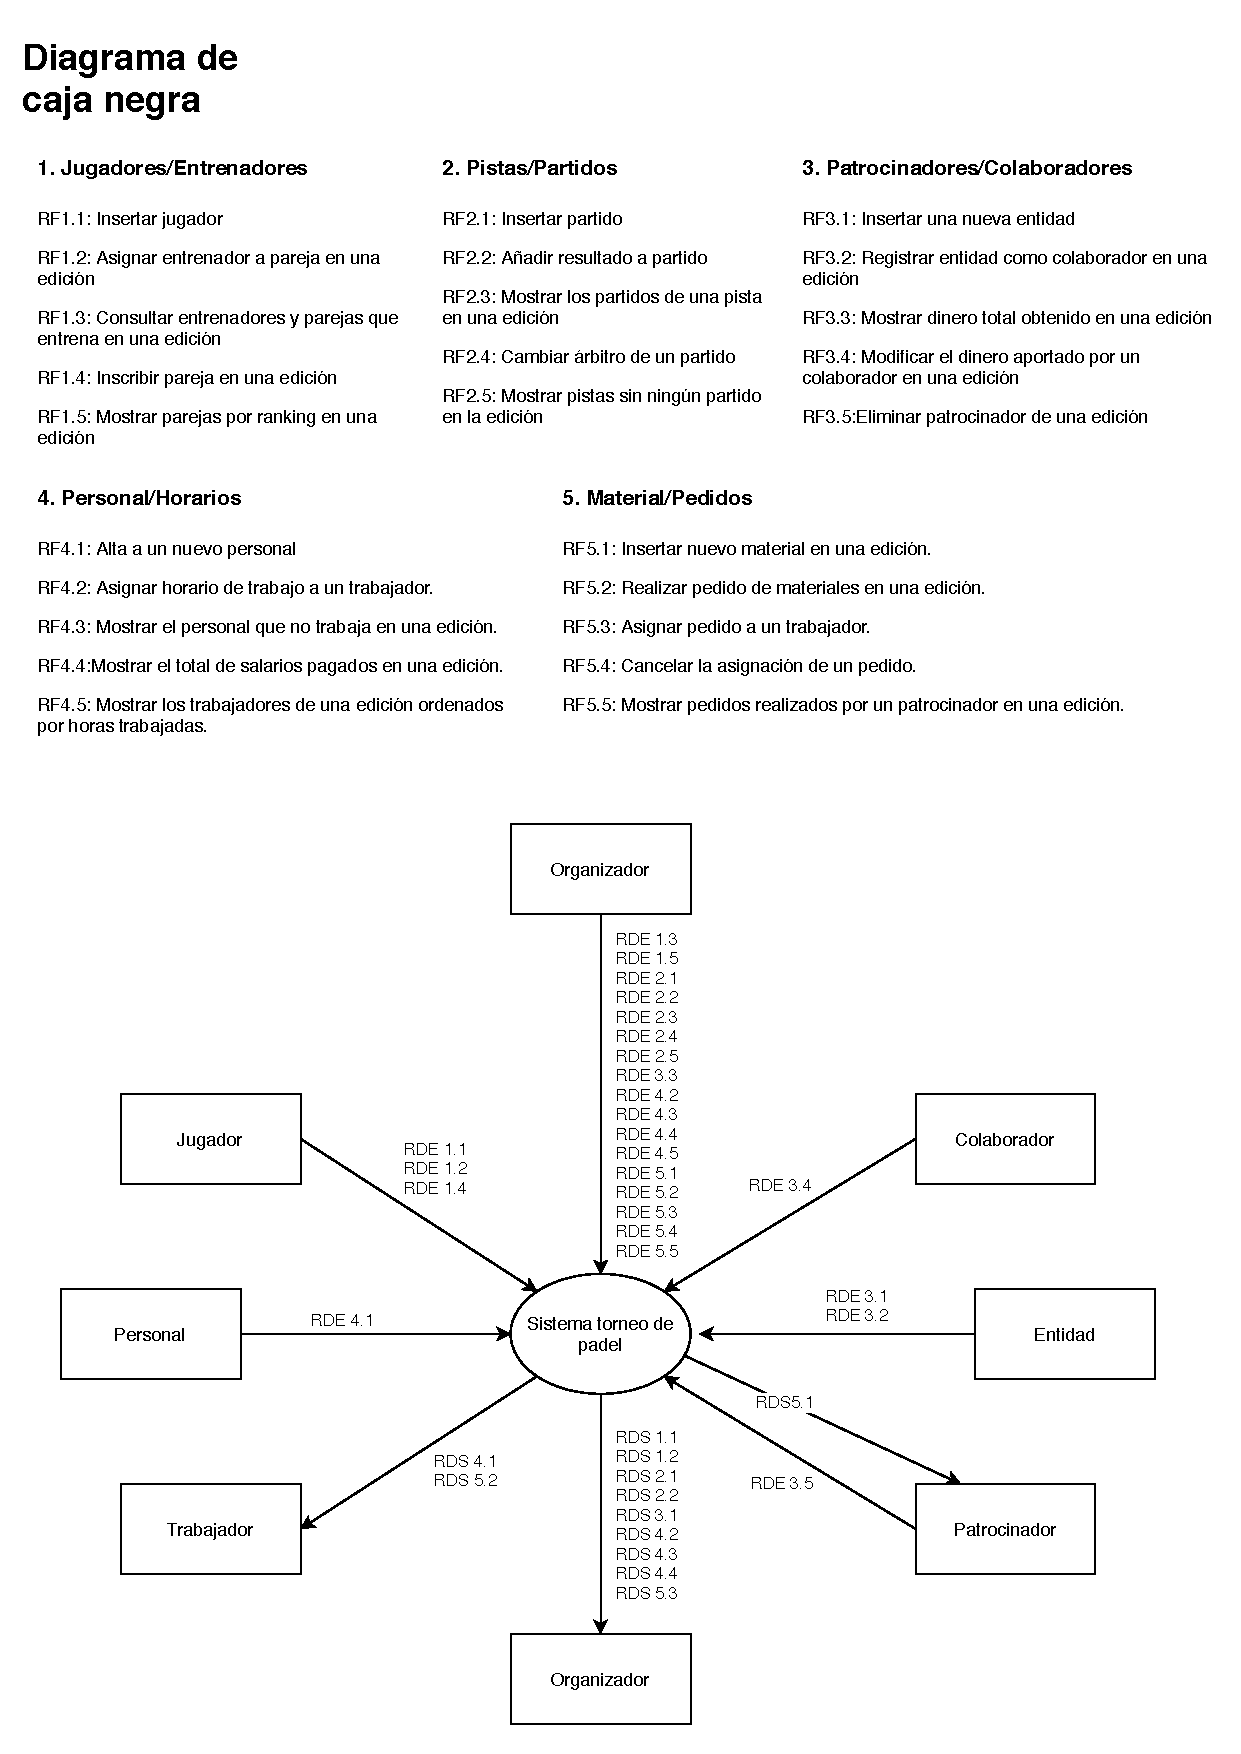
\includegraphics[height=22cm, page=1]{diagramas.pdf}

\includegraphics[height=22cm, page=2]{diagramas.pdf}

\includegraphics[height=22cm, page=3]{diagramas.pdf}

\includegraphics[height=22cm, page=4]{diagramas.pdf}

\includegraphics[height=22cm, page=5]{diagramas.pdf}

\includegraphics[height=22cm, page=6]{diagramas.pdf}

\includegraphics[height=22cm, page=7]{diagramas.pdf}

\vfill

\chapter{Diseño de datos}
\vfill
	\section{Diagramas externos}

\subsection{Jugadores-entrenadores: Clara María Romero Lara}

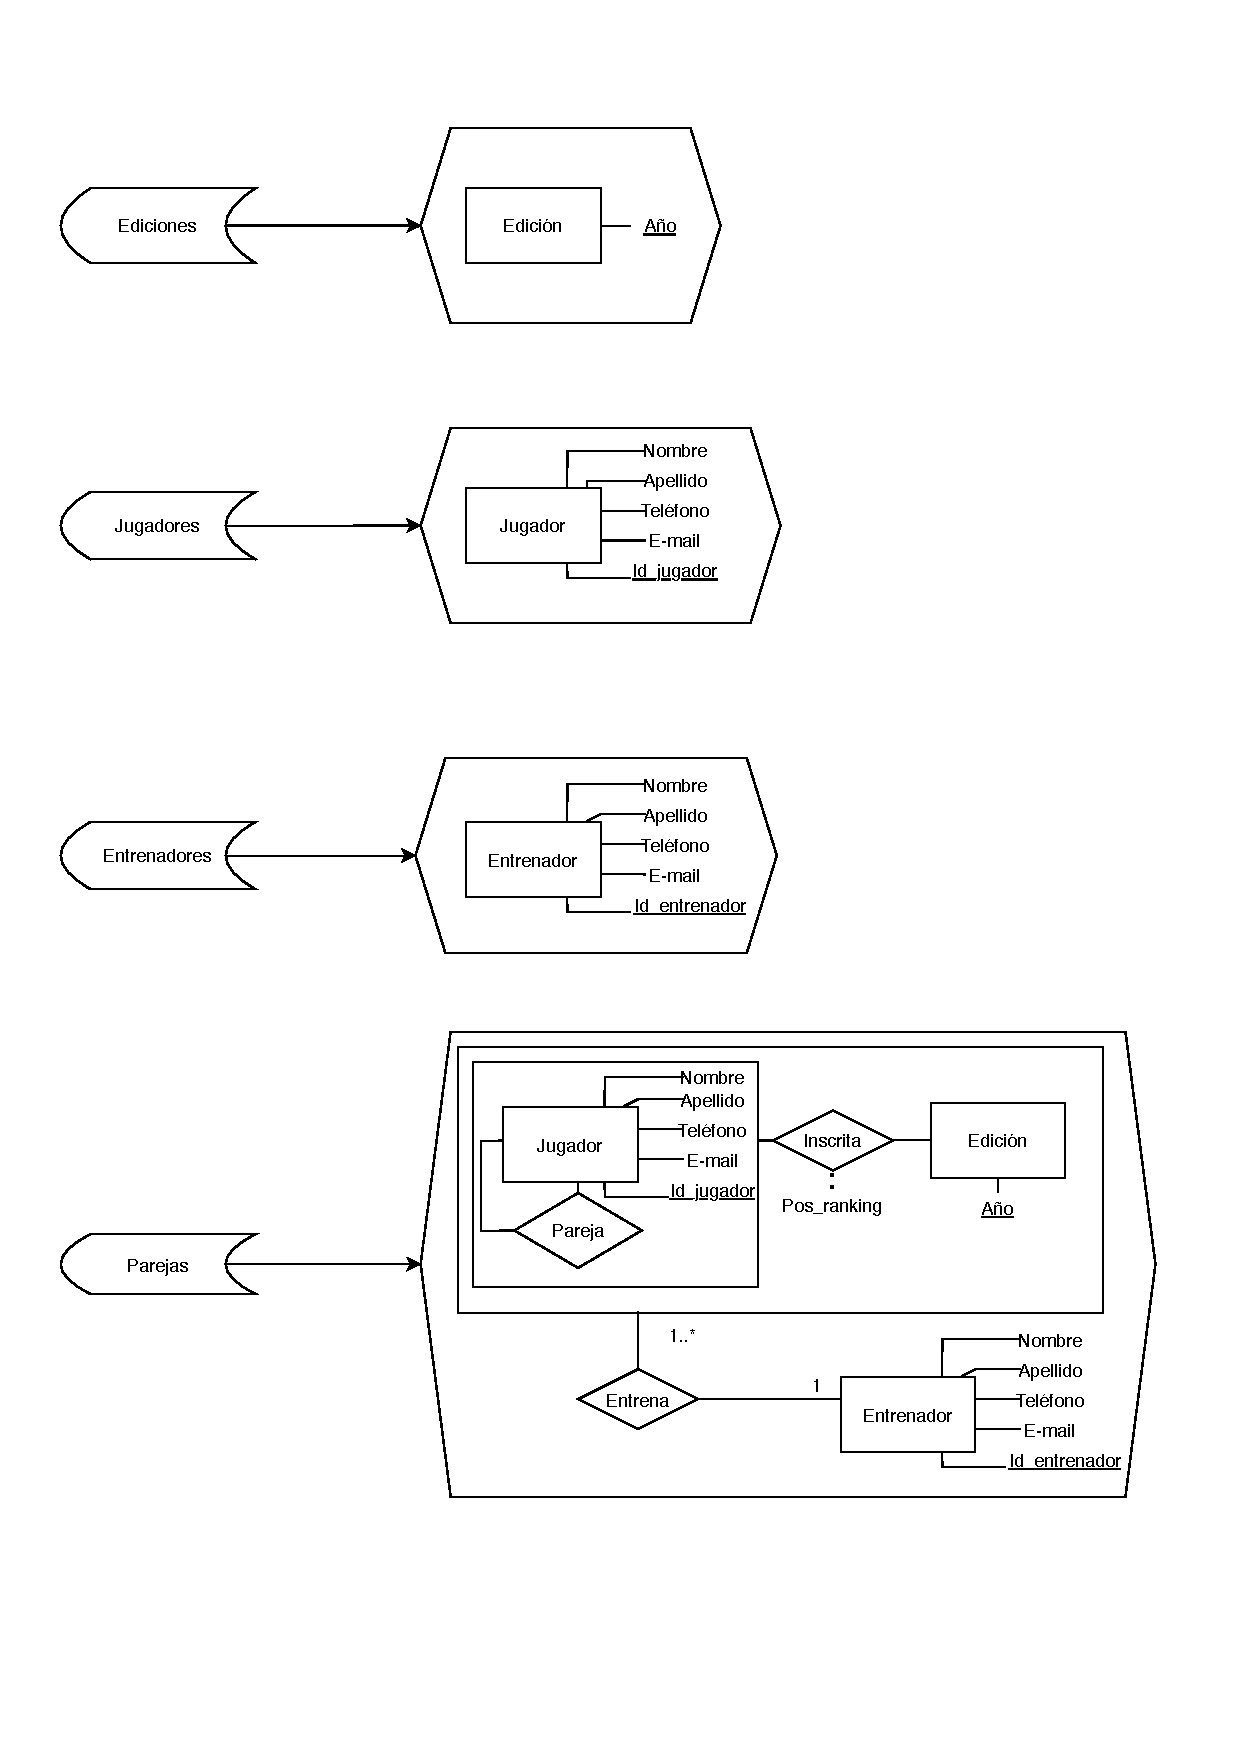
\includegraphics[height=18cm, page=1]{jug-entr.pdf}

\includegraphics[height=25cm, page=2]{jug-entr.pdf}

\includegraphics[height=25cm, page=3]{jug-entr.pdf}

\pagebreak
\subsection{Pistas-partidos: Javier Expósito Martínez}

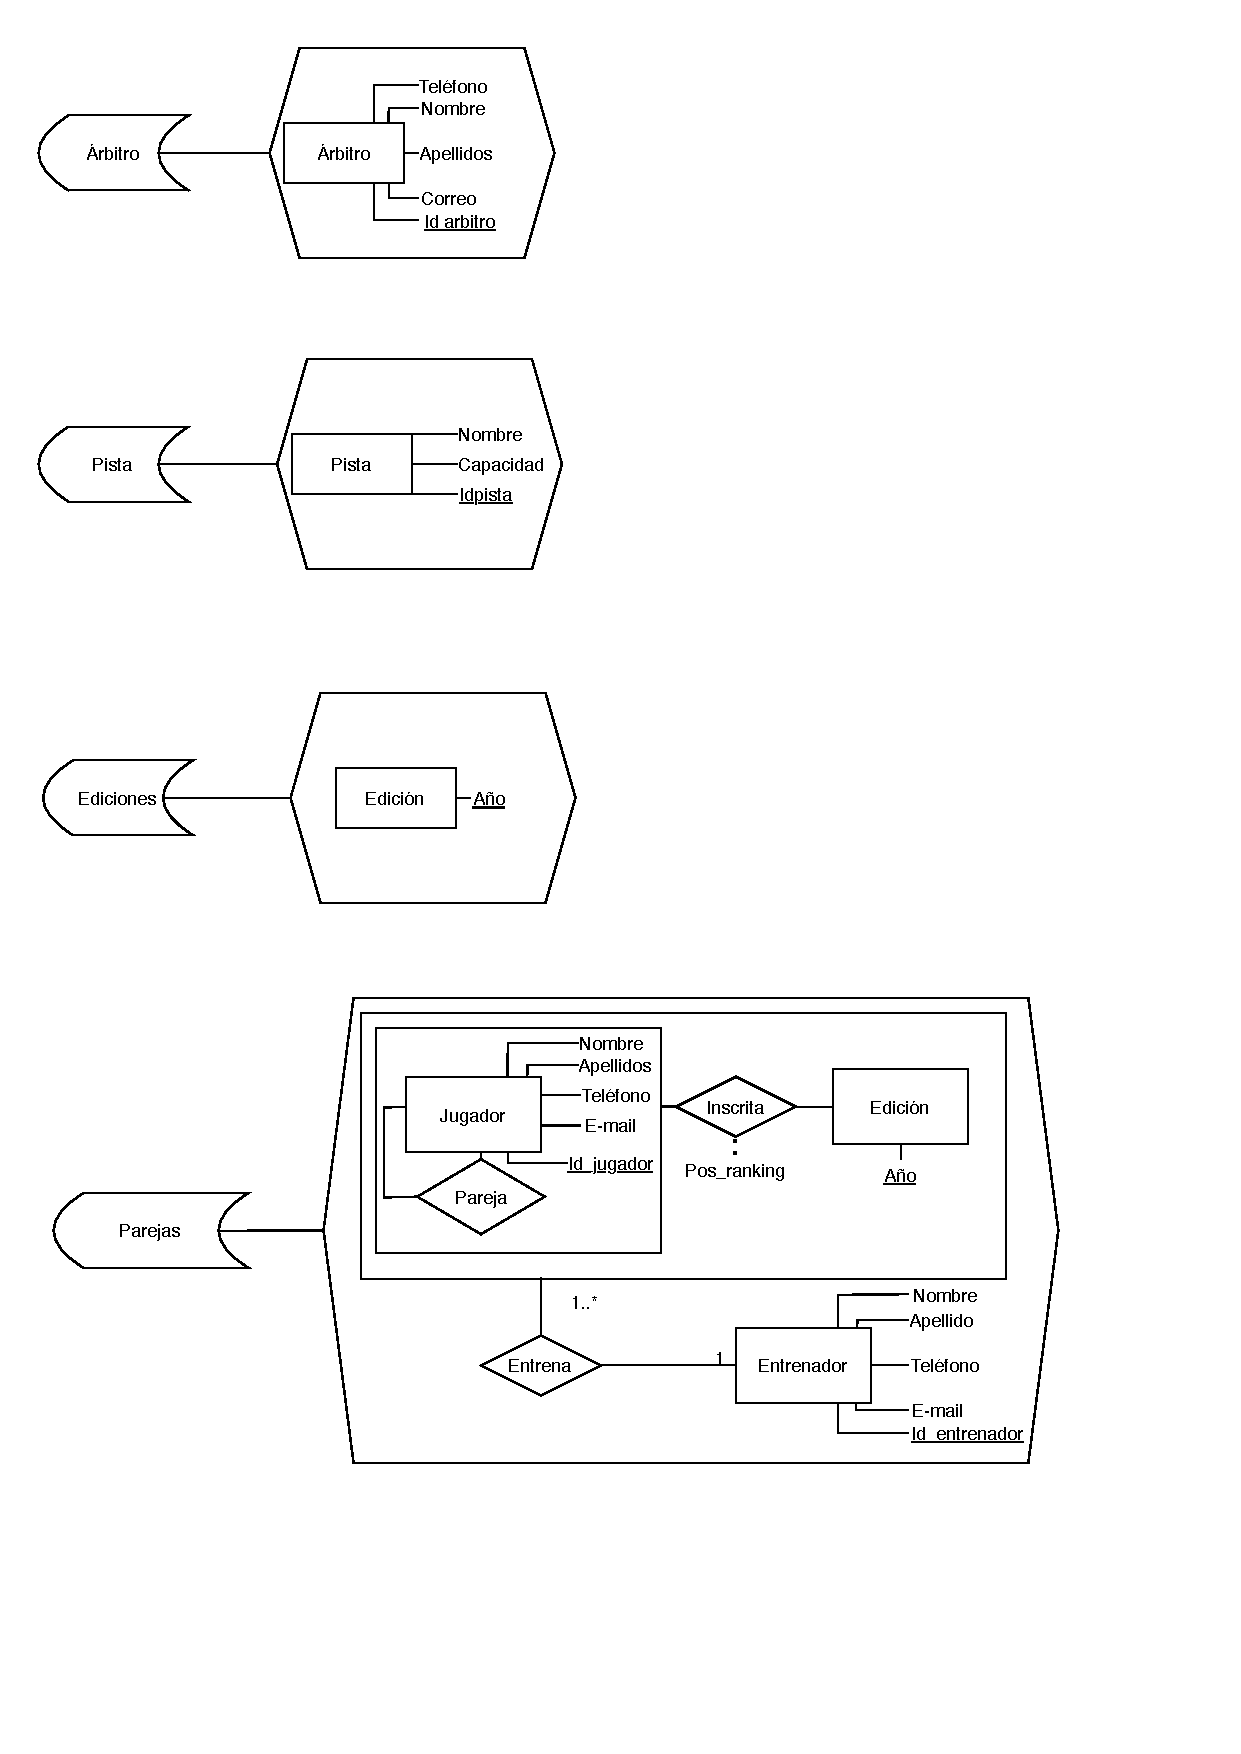
\includegraphics[height=18cm, page=1]{pist-part.pdf}

\includegraphics[height=20cm, page=2]{pist-part.pdf}

\includegraphics[height=25cm, page=3]{pist-part.pdf}

\includegraphics[height=25cm, page=4]{pist-part.pdf}

\includegraphics[height=25cm, page=5]{pist-part.pdf}


\subsection{Patrocinadores-colaboradores: Leire Requena Garcia}

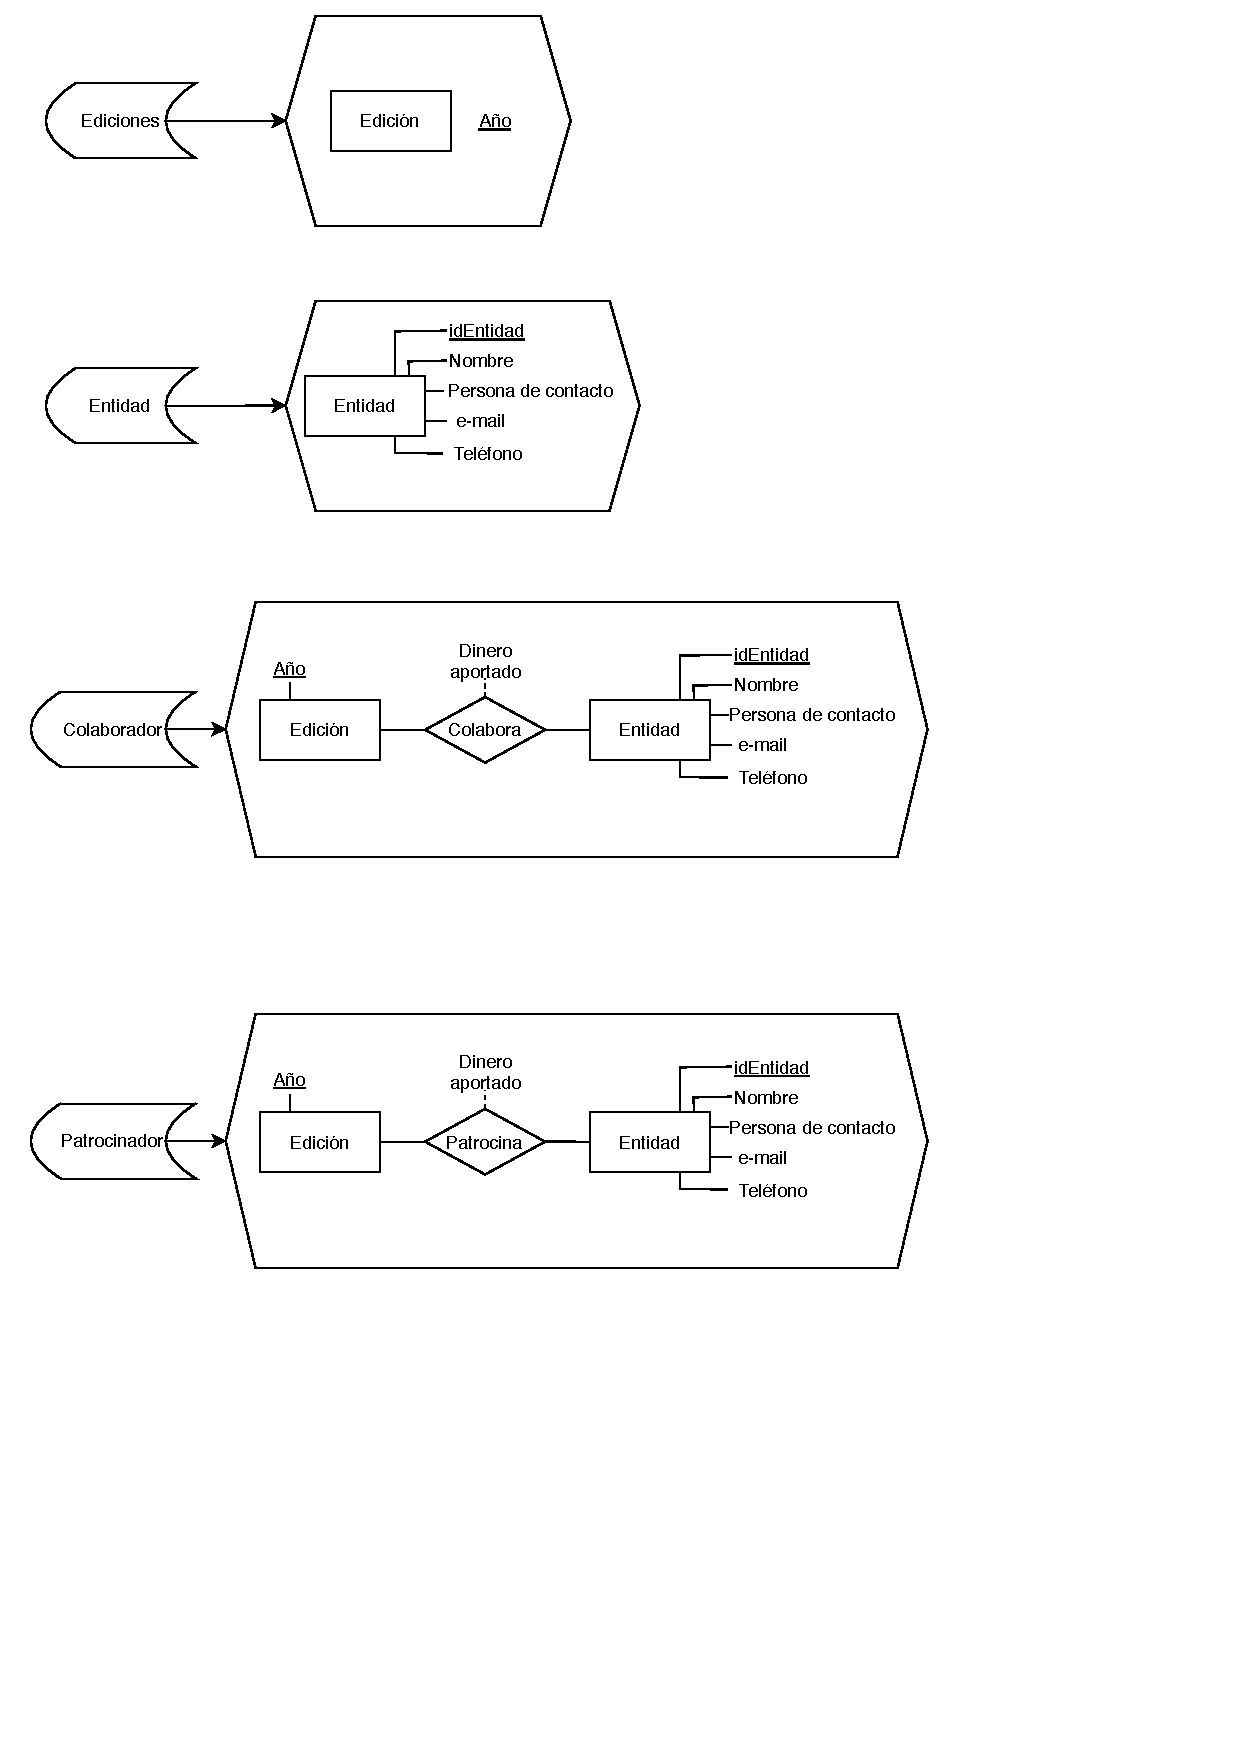
\includegraphics[height=25cm,page=1]{patr-col.pdf}

\includegraphics[height=25cm,page=2]{patr-col.pdf}

\pagebreak

\subsection{Personal-horarios: Laura Sánchez Sánchez}

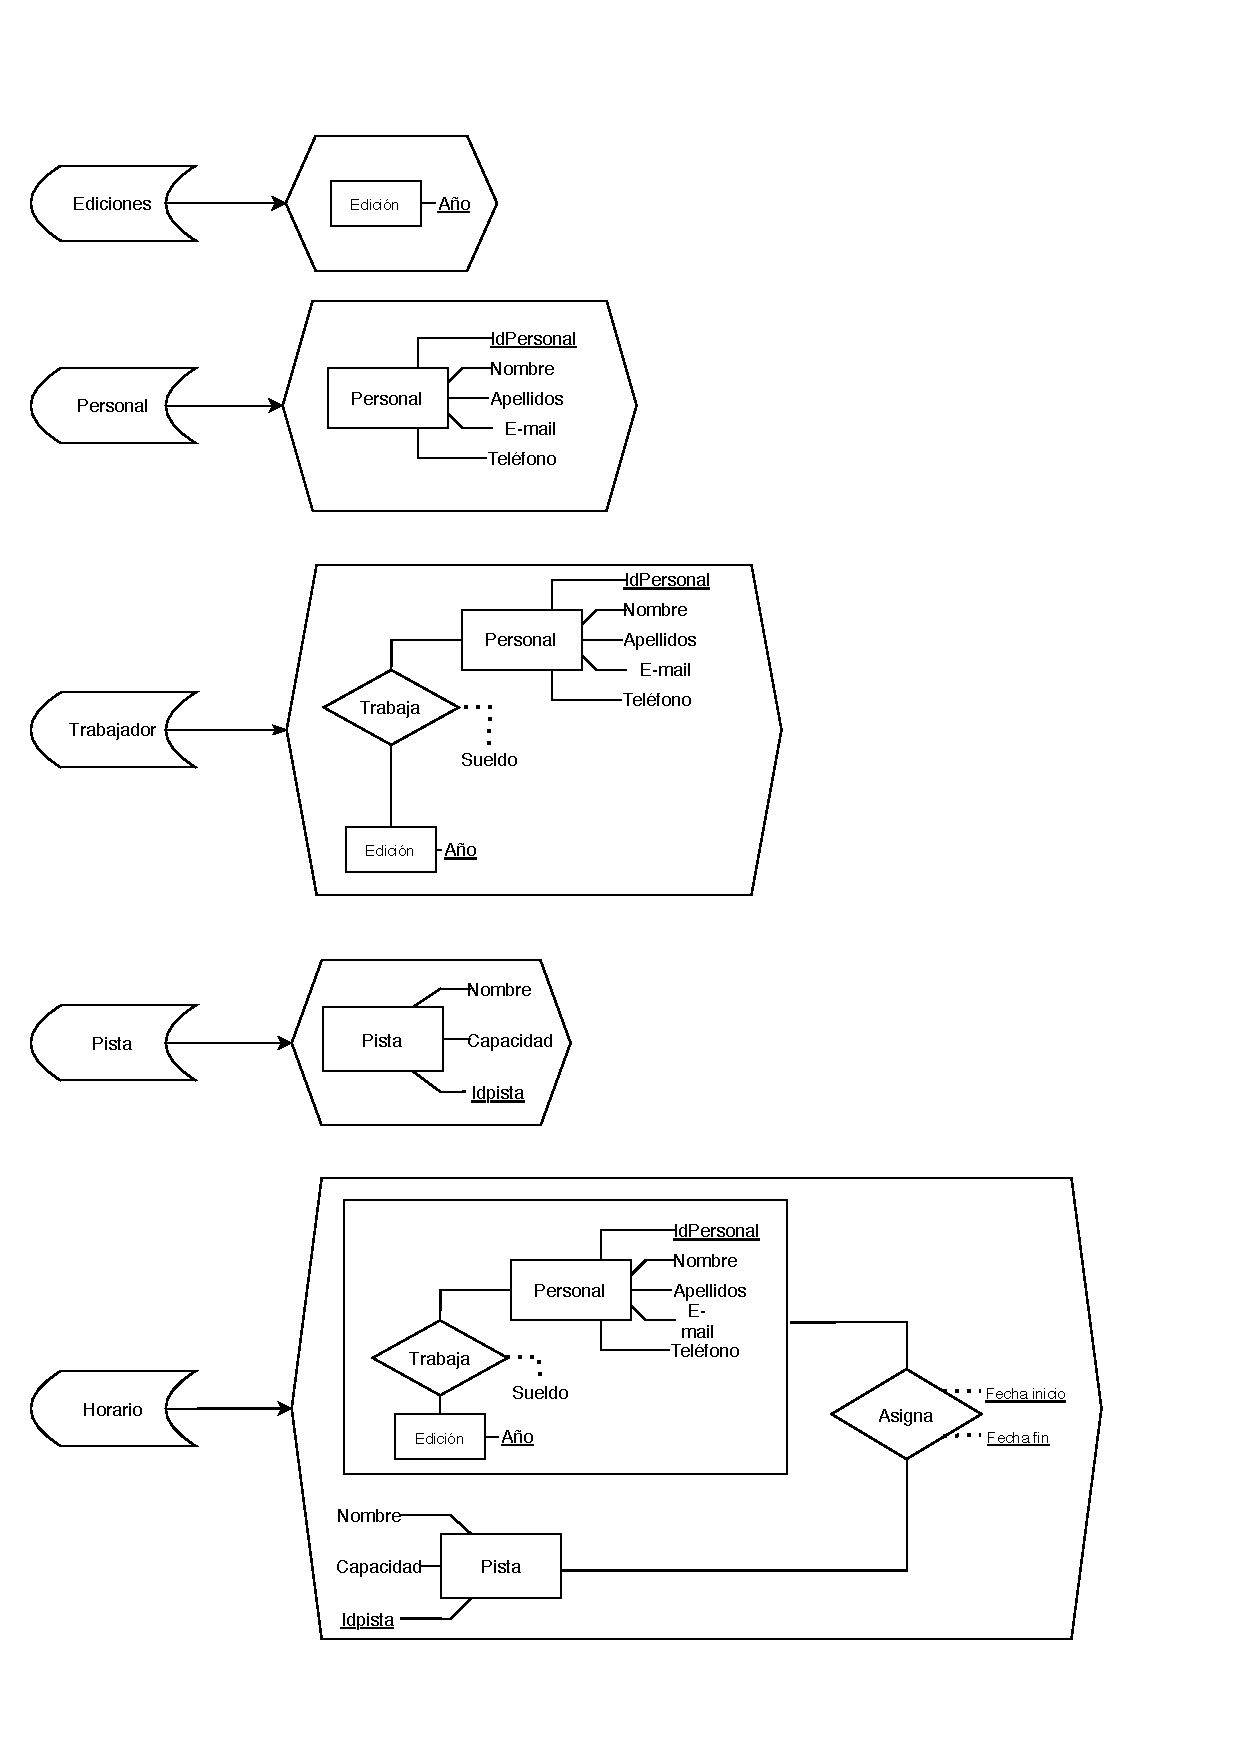
\includegraphics[height=20cm,page=1]{per-hor.pdf}

\includegraphics[height=25cm,page=2]{per-hor.pdf}

\includegraphics[height=25cm,page=3]{per-hor.pdf}

\subsection{Materiales-pedidos: Inés Nieto Sánchez}

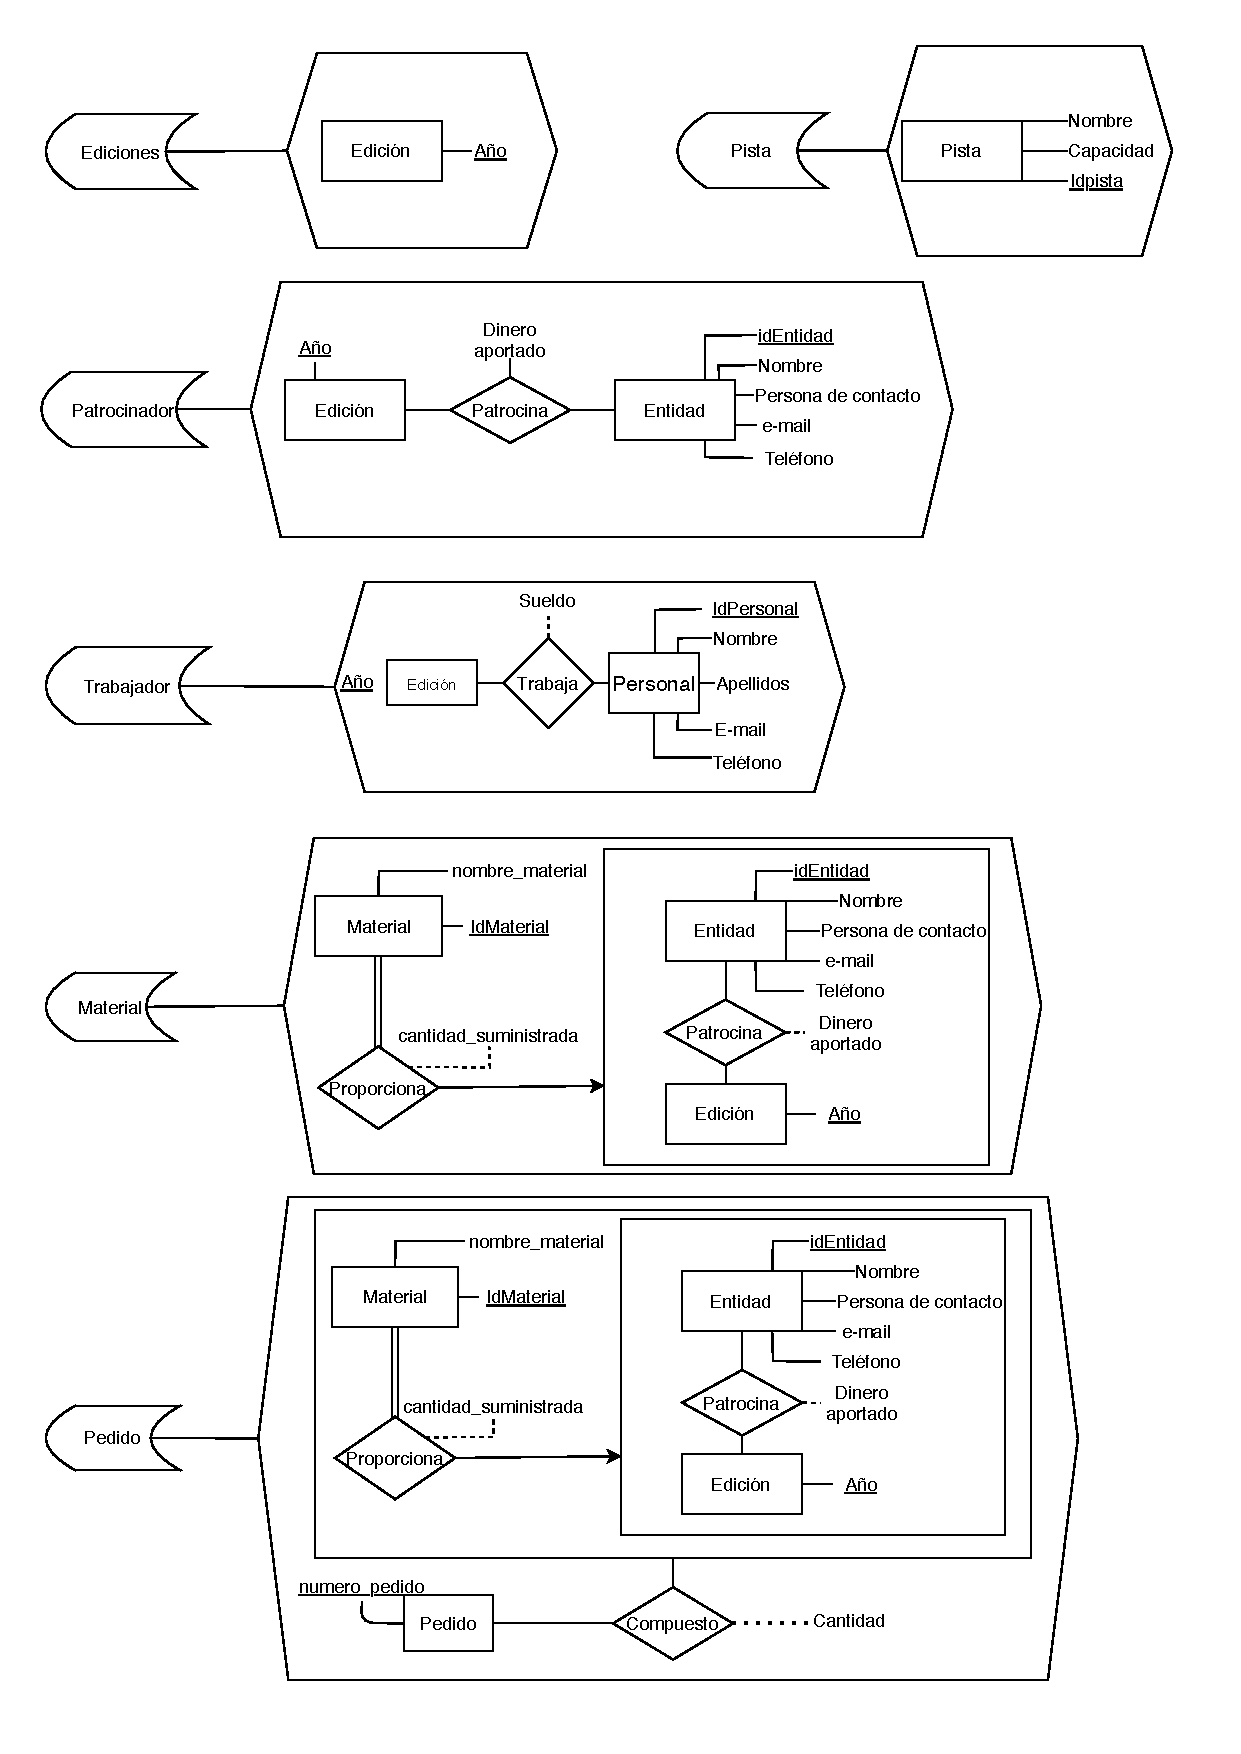
\includegraphics[height=20cm, page=1]{mat-ped.pdf}

\includegraphics[height=25cm, page=2]{mat-ped.pdf}

\includegraphics[height=25cm, page=3]{mat-ped.pdf}

	\pagebreak
	\begin{landscape}
\section{Diagrama entidad/relación}
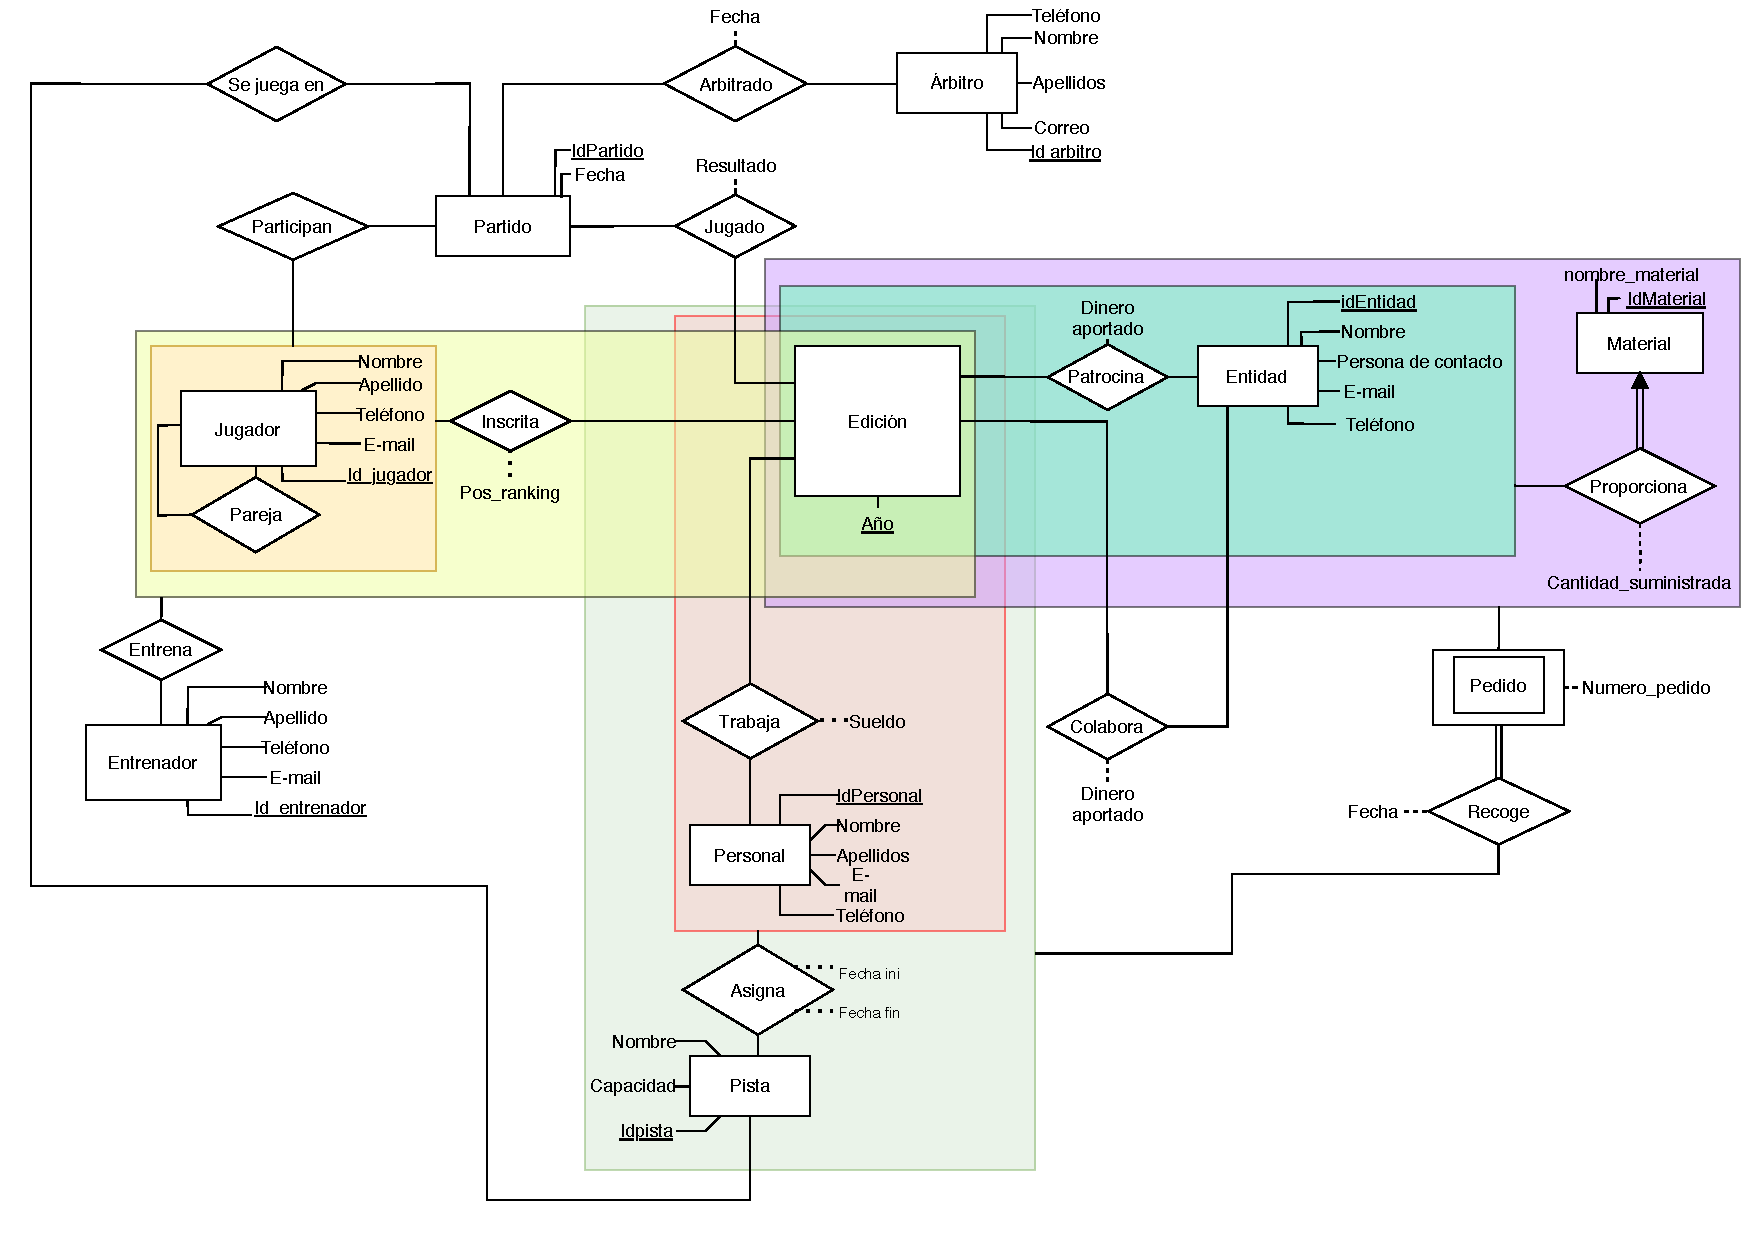
\includegraphics[height=15cm]{E_R.pdf}
\end{landscape}
	\pagebreak
	\section{Paso a tablas}
\subsubsection{Leyenda}
\begin{itemize}
	\item Para indicar una clave primaria esta se \underline{subrayará}.
	\item Para indicar una clave externa se acompañará de CE y el número de la tabla de la que viene la clave.
	\item Para indicar una clave compuesta se encerrará entre corchetes [].
\end{itemize}

\subsubsection{Tablas}
\begin{enumerate}
	\item \textbf{Edición: } (\underline{Año})
	\item \textbf{Jugador: } (\underline{idJugador}, nombreJ, apellidoJ, teléfonoJ, e-mailJ)
	\item \textbf{Entrenador: } (\underline{idEntrenador}, nombreE, apellidoE, teléfonoE, e-mailE)
	\item \textbf{Partido: } (\underline{idPartido}, fecha, resultado)
	\item \textbf{Árbitro: } (\underline{idÁrbitro}, nombreA, apellidoA, teléfonoA,e-mailA)
	\item \textbf{Personal: } (\underline{idPersonal}, nombreP, apellidosP, e-mailP, teléfonoP)
	\item \textbf{Pista: } (\underline{idPista}, nombre, capacidad)
	\item \textbf{Entidad: } (\underline{idEntidad}, nombreEn, persona de contacto, e-mailEn, teléfonoEn)
	\item \textbf{Material: } (\underline{idMaterial}, nombre\_material)
	\item \textbf{Pedido: } (\underline{Numero\_pedido})
\newline
	\item \textbf{Se juega en: } (\underline{idPartido CE4}, idPista CE7)
	\item \textbf{Arbitrado: } (\underline{idPartido CE4}, idArbitro CE5)
	\item \textbf{Participan: } (\underline{[[idJugador, idJugador], Año] CE16, idPartido CE4})
	\item \textbf{Jugado: } (\underline{idPartido CE4}, idAño CE1)
	\item \textbf{Pareja: } (\underline{[idJugador CE 2, idJugador CE 2]})
	\item \textbf{Inscrita: } (\underline{[[idJugador, idJugador] CE 15, Año CE 1]}, pos\_ranking)
	\item \textbf{Entrena: } (\underline{[[[[idJugador, idJugador] CE 15, Año CE 1] CE 16], idEntrenador CE 3]})
	\item \textbf{Trabaja: } (\underline{[idPersonal CE6, año CE1]}, sueldo)
	\item \textbf{Asigna: } (\underline{[[idPersonal, año]CE18, idPista CE7, FechaInicio, FechaFin]})
	\item \textbf{Colabora: } (\underline{[idEntidad CE8, Año CE 1]}, dinero aportado)
	\item \textbf{Patrocina: } (\underline{[idEntidad CE8, Año CE 1]}, dinero aportado)
	\item \textbf{Proporciona: } (\underline{idMaterial CE 9}, [idEntidad, Año]CE21, Cantidad\_suministrada)
	\item \textbf{Recoge: } (\underline{Numero\_pedido CE 10},[[idPersonal, año], idPista, FechaInicio, FechaFin]CE19, Fecha)
	\item \textbf{Compuesto: } (\underline{[idMaterial CE 22, Numero\_pedido CE 10]}, Cantidad)
\end{enumerate}

\subsection{Normalización}
En este caso, las tablas no han sufrido ningún cambio durante el proceso de normalización
porque el diseño era correcto y nuestras tablas, desde un principio, se encontraban en
forma normal de Boyce-Codd.

\subsubsection{2FN}
La segunda forma normal se cumplía: todos los atributos no primos de las tablas dependen de las claves candidatas.
Dado que en cada tabla sólo hay una clave candidata, estos atributos no primos dependen de ella, la clave primaria.


\subsubsection{3FN}
También cumplíamos los requisitos de la tercera forma normal: está en segunda forma normal;
y no existe ninguna dependencia transitiva problemática (tipo A \rightarrow B, B \rightarrow C, C \rightarrow !A). Esto se debe a
que, como hemos explicado, todos los atributos no primos sólo dependen de la clave primaria, y no
hay ninguno que dependa de algo que no sea la clave.


\subsubsection{FNBC}
En el caso de la forma normal de Boyce-Codd, no hay más que una clave candidata, por lo que no
hay claves candidatas compuestas que tengan atributos en común.

	\pagebreak
	\pagebreak
\section{Sentencias SQL}
\subsection{Creación de tablas}
\begin{lstlisting}[language=sql]
CREATE TABLE Edicion(
	Año INT,
	PRIMARY KEY (Año)
);

CREATE TABLE Jugador(
	idJugador INT,
	nombreJ VARCHAR(30),
	apellidoJ VARCHAR(60),
	telefonoJ VARCHAR(12) CONSTRAINT tfnoJ CHECK(regexp_like(telefonoJ,'^[/+]?[0-9]')),
	emailJ VARCHAR(50) CONSTRAINT mail_checkJ CHECK (emailJ LIKE '%_@__%.__%'),
	PRIMARY KEY (idJugador)
);

CREATE TABLE Entrenador(
	idEntrenador INT,
	nombreE VARCHAR(30),
	apellidoE VARCHAR(60),
	telefonoE VARCHAR(12) CONSTRAINT tfnoE CHECK(regexp_like(telefonoE,'^[/+]?[0-9]')),
	emailE VARCHAR(50) CONSTRAINT mail_checkE CHECK (emailE LIKE '%_@__%.__%'),
	PRIMARY KEY (idEntrenador)
);

CREATE TABLE Partido(
	idPartido INT,
	fecha DATE,
	resultado INT,
	PRIMARY KEY (idPartido)
);

CREATE TABLE Arbitro(
	idArbitro INT,
	nombreA VARCHAR(30),
	apellidoA VARCHAR(60),
	telefonoA VARCHAR(12) CONSTRAINT tfnoA CHECK(regexp_like(telefonoA,'^[/+]?[0-9]')),
	emailA VARCHAR(50) CONSTRAINT mail_checkA CHECK (emailA LIKE '%_@__%.__%'),
	PRIMARY KEY (idArbitro)
);

CREATE TABLE Personal(
	idPersonal INT,
	nombreP VARCHAR(30),
	apellidosP VARCHAR(60),
	telefonoP VARCHAR(12) CONSTRAINT tfnoP CHECK(regexp_like(telefonoP,'^[/+]?[0-9]')),
	emailP VARCHAR(50) CONSTRAINT mail_checkP CHECK (emailP LIKE '%_@__%.__%'),
	PRIMARY KEY (idPersonal)
);

CREATE TABLE Pista(
	idPista INT,
	nombre VARCHAR(30),
	capacidad INT,
	PRIMARY KEY (idPista)
);

CREATE TABLE Entidad(
	idEntidad INT,
	nombreEn VARCHAR(30),
	persona_de_contacto VARCHAR(80),
	telefonoEn VARCHAR(12) CONSTRAINT tfnoEn CHECK(regexp_like(telefonoEn,'^[/+]?[0-9]')),
	emailEn VARCHAR(50) CONSTRAINT mail_checkEn CHECK (emailEn LIKE '%_@__%.__%'),
	PRIMARY KEY (idEntidad)
);

CREATE TABLE Material(
	idMaterial INT,
	nombre VARCHAR(30),
	PRIMARY KEY (idMaterial)
);

CREATE TABLE Pedido(
	numero_pedido INT,
	PRIMARY KEY (numero_pedido)
);

CREATE TABLE SeJuegaEN(
	idPartido INT CONSTRAINT idPartido_no_nulo NOT NULL,
	idPista INT CONSTRAINT idPista_no_nula NOT NULL,
	CONSTRAINT idPartido_clave_primaria PRIMARY KEY(idPartido),
	CONSTRAINT idPartido_clave_externa FOREIGN KEY(idPartido) REFERENCES Partido(idPartido),
	CONSTRAINT idPista_clave_externa FOREIGN KEY(idPista) REFERENCES Pista(idPista)
);

CREATE TABLE Arbitrado(
	idPartido INT CONSTRAINT idPartidoA_no_nulo NOT NULL,
	idArbitro INT CONSTRAINT idArbitro_no_nula NOT NULL,
	CONSTRAINT idPartidoA_clave_primaria PRIMARY KEY(idPartido),
	CONSTRAINT idPartidoA_clave_externa FOREIGN KEY(idPartido) REFERENCES Partido(idPartido),
	CONSTRAINT idArbitro_clave_externa FOREIGN KEY(idArbitro) REFERENCES Arbitro(idArbitro)
);

CREATE TABLE Pareja(
	idJugador1 INT,
	idJugador2 INT,
	FOREIGN KEY(idJugador1) REFERENCES Jugador(idJugador),
	FOREIGN KEY(idJugador2) REFERENCES Jugador(idJugador),
	PRIMARY KEY (idJugador1, idJugador2)
);

CREATE TABLE Inscrita(
	idJugador1 INT,
	idJugador2 INT,
	Año INT,
	Pos_ranking INT,
	FOREIGN KEY(idJugador1, idJugador2) REFERENCES Pareja(idJugador1, idJugador2),
	FOREIGN KEY(Año) REFERENCES Edicion(Año),
	PRIMARY KEY (idJugador1, idJugador2, Año)
);

CREATE TABLE Participan(
	idJugador1 INT CONSTRAINT jugadorP1_no_nulo NOT NULL,
	idJugador2 INT CONSTRAINT jugadorP2_no_nulo NOT NULL,
	Año INT CONSTRAINT Año_no_nuloP NOT NULL,
	idPartido INT CONSTRAINT Partido_no_nuloP NOT NULL,
	CONSTRAINT idClaveExterna_Inscrita FOREIGN KEY(idJugador1,idJugador2,Año)
		REFERENCES Inscrita(idJugador1,idJugador2,Año),
	CONSTRAINT idPartidoP_clave_externa FOREIGN KEY(idPartido)
		REFERENCES Partido(idPartido),
	CONSTRAINT clave_primaria_compuestaP PRIMARY KEY (idJugador1, idJugador2, Año,idPartido)

);

CREATE TABLE Jugado(
	idPartido INT CONSTRAINT idPartidoJ_no_nulo NOT NULL,
	Año INT CONSTRAINT idAño_no_nulo NOT NULL,
	CONSTRAINT idPartidoJ_clave_primaria PRIMARY KEY(idPartido),
	CONSTRAINT idPartidoJ_clave_externa FOREIGN KEY(idPartido) REFERENCES Partido(idPartido),
	CONSTRAINT idAño_clave_externa FOREIGN KEY(Año) REFERENCES Edicion(Año)
);

CREATE TABLE Entrena(
	idJugador1 INT,
	idJugador2 INT,
	idEntrenador INT,
	Año INT,
	FOREIGN KEY(idJugador1,idJugador2, Año) REFERENCES Inscrita(idJugador1,idJugador2, Año),
	FOREIGN KEY(idEntrenador) REFERENCES Entrenador(idEntrenador),
	PRIMARY KEY (idJugador1, idJugador2, Año, idEntrenador)
);

CREATE TABLE Trabaja (
	idPersonal INT,
	Año INT,
	sueldo INT,
	FOREIGN KEY (idPersonal) REFERENCES Personal (idPersonal),
	FOREIGN KEY (Año) REFERENCES Edicion (Año),
	PRIMARY KEY (idPersonal, Año)
);

CREATE TABLE Asigna (
	idPersonal INT,
	Año INT,
	idPista INT,
	FechaInicio TIMESTAMP,
	FechaFin TIMESTAMP,
	FOREIGN KEY (idPersonal, Año) REFERENCES Trabaja (idPersonal, Año),
	CHECK (FechaFin > FechaInicio),
	CHECK (FechaFin > FechaInicio),
	CHECK ((CAST (FechaFin as DATE) - CAST (FechaInicio as DATE))*24< 8),
	FOREIGN KEY (idPista) REFERENCES Pista (idPista),
	PRIMARY KEY (idPersonal, Año, idPista, FechaInicio, FechaFin)
);

CREATE TABLE Colabora (
	idEntidad INT,
	Año INT,
	dinero_aportado INT,
	FOREIGN KEY(idEntidad) REFERENCES Entidad(idEntidad),
	FOREIGN KEY (Año) REFERENCES Edicion(Año),
	PRIMARY KEY (idEntidad, Año)
);

CREATE TABLE Patrocina (
	idEntidad INT,
	Año INT,
	dinero_aportado INT,
	FOREIGN KEY(idEntidad) REFERENCES Entidad(idEntidad),
	FOREIGN KEY (Año) REFERENCES Edicion(Año),
	PRIMARY KEY (idEntidad, Año)
);

CREATE TABLE Proporciona(
	idmaterial INT PRIMARY KEY,
	identidad INT,
	Año INT,
	cantidad_suministrada INT,
	FOREIGN KEY(identidad,Año) REFERENCES Patrocina(identidad,Año),
	FOREIGN KEY(idmaterial) REFERENCES Material(idmaterial)
);

CREATE TABLE Recoge(
	numero_pedido INT,
	idPersonal INT,
	Año INT,
	idPista INT,
	fechainicio TIMESTAMP,
	fechafin TIMESTAMP,
	fecha TIMESTAMP,
	CONSTRAINT CHK_Fecha CHECK (fechainicio < fechafin),
	CONSTRAINT CHK_Fecha_Recogida1 CHECK(fecha >= fechainicio AND fecha <= fechafin),
	FOREIGN KEY(numero_pedido)REFERENCES Pedido(numero_pedido),
	FOREIGN KEY(fechainicio,fechafin,idPersonal,Año, idPista)
	REFERENCES Asigna(fechainicio, fechafin, idPersonal, Año, idPista),
	PRIMARY KEY(numero_pedido)
);

CREATE TABLE Compuesto(
	idMaterial INT,
	numero_pedido INT,
	cantidad int,
	FOREIGN KEY(idMaterial) REFERENCES Proporciona(idMaterial),
	FOREIGN KEY(numero_pedido) REFERENCES Pedido(numero_pedido),
	PRIMARY KEY(idMaterial,numero_pedido)
);
\end{lstlisting}

\pagebreak
\section{Inserción en las tablas}
\subsection{Edición}
\begin{lstlisting}[language=sql]
INSERT INTO Edicion (Año) VALUES (2015);

INSERT INTO Edicion (Año) VALUES (2016);

INSERT INTO Edicion (Año) VALUES (2020);

INSERT INTO Edicion (Año) VALUES (2019);
\end{lstlisting}

\subsection{Jugador}
\begin{lstlisting}[language=sql]
INSERT INTO Jugador(idJugador,nombreJ, apellidoJ, telefonoJ, emailJ)
VALUES ('1','Juan','Perez','999000999','juan@gmail.com');

INSERT INTO Jugador(idJugador,nombreJ, apellidoJ, telefonoJ, emailJ)
VALUES ('2','Paco','Fiestas','999111999','paco@gmail.com');

INSERT INTO Jugador(idJugador,nombreJ, apellidoJ, telefonoJ, emailJ)
VALUES ('3','Mari','Gomez','999222999','mari@gmail.com');

INSERT INTO Jugador(idJugador,nombreJ, apellidoJ, telefonoJ, emailJ)
VALUES ('4','Sara','Sarao','999333999','sara@gmail.com');

\end{lstlisting}

\subsection{Entrenador}
\begin{lstlisting}[language=sql]
INSERT INTO Entrenador(idEntrenador, nombreE,apellidoE,telefonoE,emailE)
VALUES (1, 'Alberto', 'Lopez', '342567687', 'albi@gmail.com');

INSERT INTO Entrenador(idEntrenador, nombreE,apellidoE,telefonoE,emailE)
VALUES (2, 'Miguel', 'Morena', '754756386', 'morc@gmail.com');

INSERT INTO Entrenador(idEntrenador, nombreE,apellidoE,telefonoE,emailE)
VALUES (3, 'Pedro', 'Hidalgo', '456789853', 'pdrh@gmail.com');

INSERT INTO Entrenador(idEntrenador, nombreE,apellidoE,telefonoE,emailE)
VALUES (4, 'Curro', 'Toledano', '124567890', 'Curreoat@gmail.com');
\end{lstlisting}

\subsection{Partido}
\begin{lstlisting}[language=sql]
INSERT INTO Partido(idPartido,fecha,resultado)
VALUES(1,TO_TIMESTAMP('2016-08-06 08:14:00.742000000', 'YYYY-MM-DD HH24:MI:SS.FF'),'1-5');

INSERT INTO Partido(idPartido,fecha,resultado)
VALUES(2,TO_TIMESTAMP('2015-08-07 08:15:00.742000000', 'YYYY-MM-DD HH24:MI:SS.FF'),'2-2');

INSERT INTO Partido(idPartido,fecha)
VALUES(3,TO_TIMESTAMP('2020-08-08 08:16:00.742000000', 'YYYY-MM-DD HH24:MI:SS.FF'));

INSERT INTO Partido(idPartido,fecha,resultado)
VALUES(4,TO_TIMESTAMP('2019-08-09 08:17:00.742000000', 'YYYY-MM-DD HH24:MI:SS.FF'),'4-3');
\end{lstlisting}

\pagebreak

\subsection{Árbitro}
\begin{lstlisting}[language=sql]
INSERT INTO Arbitro(idArbitro, nombreA,apellidoA,telefonoA,emailA)
VALUES (1, 'Luis', 'de Haro', '593591125', 'ajskd@gmail.com');

INSERT INTO Arbitro(idArbitro, nombreA,apellidoA,telefonoA,emailA)
VALUES (2, 'Raul', 'Gonzalez', '123567659', 'qwasdew@gmail.com');

INSERT INTO Arbitro(idArbitro, nombreA,apellidoA,telefonoA,emailA)
VALUES (3, 'Enrique', 'Camacho', '456789012', 'camch@gmail.com');

INSERT INTO Arbitro(idArbitro, nombreA,apellidoA,telefonoA,emailA)
VALUES (4, 'Critina', 'Reina', '981234567', 'cris@gmail.com');
\end{lstlisting}

\subsection{Personal}
\begin{lstlisting}[language=sql]
INSERT INTO Personal (idPersonal, nombreP, apellidosP, emailP, telefonoP)
VALUES (1, 'Javier', 'Martinez Perez', 'javier@gmail.com', 12345678);

INSERT INTO Personal (idPersonal, nombreP, apellidosP, emailP, telefonoP)
VALUES (2, 'Lorena', 'Sanchez Ortega', 'lorena@gmail.com', 12995112);

INSERT INTO Personal (idPersonal, nombreP, apellidosP, emailP, telefonoP)
VALUES (3, 'Laura', 'Catena Carrasco', 'laura@gmail.com', 12345030);

INSERT INTO Personal (idPersonal, nombreP, apellidosP, emailP, telefonoP)
VALUES (4, 'Felipe', 'Fernandez Fernandez', 'felipe@gmail.com', 12300678);
\end{lstlisting}

\subsection{Pista}
\begin{lstlisting}[language=sql]
INSERT INTO Pista (idPista, nombre, capacidad) VALUES (1, 'Pista Uno', 6);

INSERT INTO Pista (idPista, nombre, capacidad) VALUES (2, 'Pista Dos', 16);

INSERT INTO Pista (idPista, nombre, capacidad) VALUES (3, 'Pista Tres', 8);

INSERT INTO Pista (idPista, nombre, capacidad) VALUES (4, 'Pista Cuatro', 7);
\end{lstlisting}

\subsection{Entidad}
\begin{lstlisting}[language=sql]
INSERT INTO Entidad(idEntidad, nombreEn, persona_de_contacto, telefonoEn, emailEn)
VALUES (1, 'Gestoría García', 'Isabel', '987546523', 'asbdsk@ddnbcls.com');

INSERT INTO Entidad(idEntidad, nombreEn, persona_de_contacto, telefonoEn, emailEn)
VALUES (2, 'Traducciones Tradurea', 'Alba', '568785234', 'qqqqqqq@ttttttt.com');

INSERT INTO Entidad(idEntidad, nombreEn, persona_de_contacto, telefonoEn, emailEn)
VALUES (3, 'Los Rigos', 'Pepel', '111223344', 'ooooooo@ddddd.com');

INSERT INTO Entidad(idEntidad, nombreEn, persona_de_contacto, telefonoEn, emailEn)
VALUES (4, 'El Señorío', 'Pablo', '777889944', 'vdr@kjdls.com');
\end{lstlisting}

\pagebreak

\subsection{Material}
\begin{lstlisting}[language=sql]
INSERT INTO Material(idMaterial,nombre) VALUES(1,'palas');

INSERT INTO Material(idMaterial,nombre) VALUES(2,'pelotas');

INSERT INTO Material(idMaterial,nombre) VALUES(3,'botellas de agua');

INSERT INTO Material(idMaterial,nombre) VALUES(4,'Toallas');
\end{lstlisting}

\subsection{Pedido}
\begin{lstlisting}[language=sql]
INSERT INTO Pedido(numero_pedido) VALUES(1);

INSERT INTO Pedido(numero_pedido) VALUES(2);

INSERT INTO Pedido(numero_pedido) VALUES(3);

INSERT INTO Pedido(numero_pedido) VALUES(4);
\end{lstlisting}

\subsection{Se juega en}
\begin{lstlisting}[language=sql]
INSERT INTO SeJuegaEN (idPartido,idPista) VALUES (1,1);

INSERT INTO SeJuegaEN (idPartido,idPista) VALUES (2,2);

INSERT INTO SeJuegaEN (idPartido,idPista) VALUES (3,3);

INSERT INTO SeJuegaEN (idPartido,idPista) VALUES (4,4);
\end{lstlisting}

\subsection{Arbitrado}
\begin{lstlisting}[language=sql]
INSERT INTO Arbitrado (idPartido,idArbitro) VALUES (1,1);

INSERT INTO Arbitrado (idPartido,idArbitro) VALUES (2,2);

INSERT INTO Arbitrado (idPartido,idArbitro) VALUES (3,3);

INSERT INTO Arbitrado (idPartido,idArbitro) VALUES (4,4);
\end{lstlisting}
\pagebreak
\subsection{Pareja}
\begin{lstlisting}[language=sql]
INSERT INTO Pareja(idJugador1, idJugador2) VALUES (1,2);

INSERT INTO Pareja(idJugador1, idJugador2) VALUES (1,3);

INSERT INTO Pareja(idJugador1, idJugador2) VALUES (1,4);

INSERT INTO Pareja(idJugador1, idJugador2) VALUES (2,1);

INSERT INTO Pareja(idJugador1, idJugador2) VALUES (2,3);

INSERT INTO Pareja(idJugador1, idJugador2) VALUES (2,4);

INSERT INTO Pareja(idJugador1, idJugador2) VALUES (3,1);

INSERT INTO Pareja(idJugador1, idJugador2) VALUES (3,2);

INSERT INTO Pareja(idJugador1, idJugador2) VALUES (3,4);

INSERT INTO Pareja(idJugador1, idJugador2) VALUES (4,1);

INSERT INTO Pareja(idJugador1, idJugador2) VALUES (4,2);

INSERT INTO Pareja(idJugador1, idJugador2) VALUES (4,3);
\end{lstlisting}

\subsection{Inscrita}
\begin{lstlisting}[language=sql]
INSERT INTO Inscrita(idJugador1, idJugador2, Año)
VALUES ('1','2','2020');

INSERT INTO Inscrita(idJugador1, idJugador2, Año)
VALUES ('3','4','2020');

INSERT INTO Inscrita(idJugador1, idJugador2, Año, Pos_ranking)
VALUES ('1','3','2015','6');

INSERT INTO Inscrita(idJugador1, idJugador2, Año, Pos_ranking)
VALUES ('2','4','2019','3');
\end{lstlisting}

\subsection{Participan}
\begin{lstlisting}[language=sql]
INSERT INTO Participan(IdJugador1,idJugador2,Año,idPartido) VALUES(1,2,2020,2);

INSERT INTO Participan(IdJugador1,idJugador2,Año,idPartido) VALUES(3,4,2020,1);

INSERT INTO Participan(IdJugador1,idJugador2,Año,idPartido) VALUES(1,3,2015,3);

INSERT INTO Participan(IdJugador1,idJugador2,Año,idPartido) VALUES(2,4,2019,4);
\end{lstlisting}

\subsection{Jugado}
\begin{lstlisting}[language=sql]
INSERT INTO Jugado (idPartido,Año) VALUES (1,2016);

INSERT INTO Jugado (idPartido,Año) VALUES (2,2015);

INSERT INTO Jugado (idPartido,Año) VALUES (3,2020);

INSERT INTO Jugado (idPartido,Año) VALUES (4,2019);
\end{lstlisting}

\subsection{Entrena}
\begin{lstlisting}[language=sql]
INSERT INTO Entrena(idJugador1, idJugador2, idEntrenador, Año)
VALUES ('1','2','1','2020');

INSERT INTO Entrena(idJugador1, idJugador2, idEntrenador, Año)
VALUES ('3','4','1','2020');

INSERT INTO Entrena(idJugador1, idJugador2, idEntrenador, Año)
VALUES ('1','3','3','2015');

INSERT INTO Entrena(idJugador1, idJugador2, idEntrenador, Año)
VALUES ('2','4','2','2019');
\end{lstlisting}

\subsection{Trabaja}
\begin{lstlisting}[language=sql]
INSERT INTO Trabaja  (idPersonal, Año, sueldo)  values (4, 2015, 950.5);

INSERT INTO Trabaja  (idPersonal, Año, sueldo)  values (2, 2016, 900.5);

INSERT INTO Trabaja  (idPersonal, Año, sueldo)  values (1, 2019, 750.5);

INSERT INTO Trabaja  (idPersonal, Año, sueldo)  values (3, 2020, 860.5);
\end{lstlisting}

\subsection{Asigna}
\begin{lstlisting}[language=sql]
INSERT INTO Asigna(idPersonal,Año,idPista,FechaInicio,FechaFin)
VALUES(3, 2020, 2,
	TO_TIMESTAMP('2020-07-02 09:00:00.742000000', 'YYYY-MM-DD HH24:MI:SS.FF'),
	TO_TIMESTAMP('2020-07-02 16:00:00.742000000', 'YYYY-MM-DD HH24:MI:SS.FF')
);

INSERT INTO Asigna(idPersonal,Año,idPista,FechaInicio,FechaFin)
VALUES(1, 2019, 2,
	TO_TIMESTAMP('2019-08-06 09:00:00.742000000', 'YYYY-MM-DD HH24:MI:SS.FF'),
	TO_TIMESTAMP('2019-08-06 16:00:00.742000000', 'YYYY-MM-DD HH24:MI:SS.FF')
	);

INSERT INTO Asigna(idPersonal,Año,idPista,FechaInicio,FechaFin)
VALUES(2, 2016, 2,
	TO_TIMESTAMP('2016-09-15 09:00:00.742000000', 'YYYY-MM-DD HH24:MI:SS.FF'),
	TO_TIMESTAMP('2016-09-15 16:00:00.742000000', 'YYYY-MM-DD HH24:MI:SS.FF')
);

INSERT INTO Asigna(idPersonal,Año,idPista,FechaInicio,FechaFin)
VALUES(2, 2016, 2,
	TO_TIMESTAMP('2016-07-02 09:00:00.742000000', 'YYYY-MM-DD HH24:MI:SS.FF'),
	TO_TIMESTAMP('2016-07-02 16:00:00.742000000', 'YYYY-MM-DD HH24:MI:SS.FF')
);
\end{lstlisting}

\pagebreak

\subsection{Colabora}
\begin{lstlisting}[language=sql]
INSERT INTO Colabora (idEntidad, Año, dinero_aportado)
VALUES (1,2020,600);

INSERT INTO Colabora (idEntidad, Año, dinero_aportado)
VALUES (3,2015,1000);

INSERT INTO Colabora (idEntidad, Año, dinero_aportado)
VALUES (2,2020,50);

INSERT INTO Colabora (idEntidad, Año, dinero_aportado)
VALUES (4,2016,150);
\end{lstlisting}

\subsection{Patrocina}
\begin{lstlisting}[language=sql]
INSERT INTO Patrocina (idEntidad, Año, dinero_aportado)
VALUES (2,2016,800);

INSERT INTO Patrocina (idEntidad, Año, dinero_aportado)
VALUES (2,2015,2000);

INSERT INTO Patrocina (idEntidad, Año, dinero_aportado)
VALUES (3,2020,600);

INSERT INTO Patrocina (idEntidad, Año, dinero_aportado)
VALUES (4,2015,250);
\end{lstlisting}

\subsection{Proporciona}
\begin{lstlisting}[language=sql]
INSERT INTO Proporciona(idmaterial,identidad,Año,cantidad_suministrada)
VALUES(1,2,2016,20);

INSERT INTO Proporciona(idmaterial,identidad,Año,cantidad_suministrada)
VALUES(2,3,2020,50);

INSERT INTO Proporciona(idmaterial,identidad,Año,cantidad_suministrada)
VALUES(3,2,2015,80);

INSERT INTO Proporciona(idmaterial,identidad,Año,cantidad_suministrada)
VALUES(4,3,2020,50);
\end{lstlisting}

\pagebreak

\subsection{Recoge}
\begin{lstlisting}[language=sql]
INSERT INTO Recoge(numero_pedido,idpersonal,Año,idpista,fechainicio,fechafin,fecha)
VALUES(1,2,2016,2,
	TO_TIMESTAMP('2018-07-02 06:14:00.742000000', 'YYYY-MM-DD HH24:MI:SS.FF'),
	TO_TIMESTAMP('2018-07-02 11:14:00.742000000', 'YYYY-MM-DD HH24:MI:SS.FF'),
	TO_TIMESTAMP('2018-07-02 06:14:00.742000000', 'YYYY-MM-DD HH24:MI:SS.FF')
);

INSERT INTO Recoge(numero_pedido,idpersonal,Año,idpista,fechainicio,fechafin,fecha)
VALUES(2,2,2016,2,
	TO_TIMESTAMP('2018-07-02 06:14:00.742000000', 'YYYY-MM-DD HH24:MI:SS.FF'),
	TO_TIMESTAMP('2018-07-02 11:14:00.742000000', 'YYYY-MM-DD HH24:MI:SS.FF'),
	TO_TIMESTAMP('2018-07-02 09:14:00.742000000', 'YYYY-MM-DD HH24:MI:SS.FF')
);

INSERT INTO Recoge(numero_pedido,idpersonal,Año,idpista,fechainicio,fechafin,fecha)
VALUES(3,1,2019,2,
	TO_TIMESTAMP('2018-08-06 08:14:00.742000000', 'YYYY-MM-DD HH24:MI:SS.FF'),
	TO_TIMESTAMP('2018-08-06 12:14:00.742000000', 'YYYY-MM-DD HH24:MI:SS.FF'),
	TO_TIMESTAMP('2018-08-06 10:14:00.742000000', 'YYYY-MM-DD HH24:MI:SS.FF')
);

INSERT INTO Recoge(numero_pedido,idpersonal,Año,idpista,fechainicio,fechafin,fecha)
VALUES(4,1,2019,2,
	TO_TIMESTAMP('2018-08-06 08:14:00.742000000', 'YYYY-MM-DD HH24:MI:SS.FF'),
	TO_TIMESTAMP('2018-08-06 12:14:00.742000000', 'YYYY-MM-DD HH24:MI:SS.FF'),
	TO_TIMESTAMP('2018-08-06 10:14:00.742000000', 'YYYY-MM-DD HH24:MI:SS.FF')
);
\end{lstlisting}

\subsection{Compuesto}
\begin{lstlisting}[language=sql]
INSERT INTO Compuesto(IdMaterial,numero_pedido,cantidad) VALUES(1,1,20);

INSERT INTO Compuesto(IdMaterial,numero_pedido,cantidad) VALUES(2,2,30);

INSERT INTO Compuesto(IdMaterial,numero_pedido,cantidad) VALUES(3,3,50);

INSERT INTO Compuesto(IdMaterial,numero_pedido,cantidad) VALUES(4,4,50);
\end{lstlisting}



\chapter{Implementación}
	\section{Software usado}
Para la realización de esta práctica hemos recuperado los archivos necesarios para
la conexión a la base de datos con JDBC.

Hemos vuelto a usar este software porque ya conocíamos los mecanismos de las
transacciones en SQL y era sencillo hacer una interfaz por terminal que pueda
manejar un usuario.

	\pagebreak
	\section{Identificación de transacciones}
\subsubsection{Jugadores/Entrenadores: Clara María Romero Lara}
Consultar entrenador y parejas que entrena en una edición \texttt{mostrarEntrenador}

\begin{lstlisting}[language=sql]
CREATE OR REPLACE PROCEDURE mostrarEntrenador(anio IN NUMBER, idEntr IN NUMBER, salida OUT CLOB)
IS
	CURSOR cEntrena IS SELECT * FROM Entrena WHERE (anio = Año) AND (idEntr=idEntrenador);
	coach Entrena%ROWTYPE;
	coach_row CLOB;
BEGIN
	salida := 'Entrenador '||idEntr||' en la edicion '||anio||' entrena:'||CHR(10);
	OPEN cEntrena;
	FETCH cEntrena INTO coach;

	WHILE (cEntrena%FOUND) LOOP
		coach_row := '   Pareja: ' || coach.idJugador1 || ' ' || coach.idJugador2;
		salida := salida || coach_row || CHR(10);
		FETCH cEntrena INTO coach;
	END LOOP;

	CLOSE cEntrena;
END;
/
\end{lstlisting}

Previa su ejecución, deberíamos:
\begin{itemize}
	\item Insertar una edición \texttt{insertarEdicion}
	\item Insertar al menos dos jugadores \texttt{insertarJugador}
	\item Registrar una pareja \texttt{registrarPareja}
	\item Registrar una pareja en una edición \texttt{registrarInscrita}
	\item Insertar un entrenador \texttt{insertarEntrenador}
	\item Asignar un entrenador a una pareja en una edición \texttt{registrarEntrena}
\end{itemize}

\subsubsection{Pistas/Partidos: Javier Expósito Martínez}
Insertar un nuevo partido \texttt{insertarPartido}.

Se registra un partido en una pista y se introduce una tupla en la tabla \texttt{Jugado}. Es decir, en las tablas \texttt{SeJuegaEn} y \texttt{Jugado}
sólo se pueden insertar tuplas si insertamos un partido.

\begin{lstlisting}[language=sql]
CREATE OR REPLACE PROCEDURE InsertarPartido(idPartido NUMBER, fecha TIMESTAMP, resultado VARCHAR2, idEdicion NUMBER, idPista NUMBER) IS
BEGIN
	INSERT INTO Partido(idPartido,fecha,resultado) VALUES (idPartido,fecha,resultado);
	 INSERT INTO SeJuegaEN(idPartido,idPista) VALUES (idPartido,idPista);
	 INSERT INTO Jugado(idPartido,Año) VALUES (idPartido,idEdicion);
END;
/
\end{lstlisting}

Previa su ejecución, deberíamos:
\begin{itemize}
	\item Insertar una edición \texttt{InsertarEdicion}
	\item Insertar una pista \texttt{InsertarPista}
\end{itemize}

\pagebreak

\subsubsection{Patrocinadores/Colaboradores: Leire Requena Garcia}
Mostrar el dinero total obtenido en una edición \texttt{mostrarRecaducacion}.

\begin{lstlisting}[language=sql]
CREATE OR REPLACE PROCEDURE mostrarRecaudacion(edicion IN NUMBER, recaudacion OUT NUMBER) IS
	RecaudacionColab INT;
	RecaudacionPatr INT;
BEGIN
	SELECT SUM(Dinero_aportado)
	INTO RecaudacionColab
	FROM Colabora
	WHERE Año=edicion;

	SELECT SUM(Dinero_aportado)
	INTO RecaudacionPatr
	FROM Patrocina
	WHERE Año=edicion;

	recaudacion := RecaudacionPatr + RecaudacionColab;
END;
/
\end{lstlisting}

Previa su ejecución, deberíamos:
\begin{itemize}
	\item Insertar una edición \texttt{insertarEdicion}
	\item Insertar una entidad \texttt{insertarEntidad}
	\item Registrar al menos un colaborador y/o un patrocinador \texttt{registrarColaborador, registrarPatrocinador}
\end{itemize}

\subsubsection{Personal/Horarios: Laura Sánchez Sánchez}
Mostrar el personal que no trabaja en una edición \texttt{mostrarPersonal}.

\begin{lstlisting}[language=sql]
CREATE OR REPLACE PROCEDURE mostrarPersonal (anio IN NUMBER, salida OUT CLOB)
IS
	CURSOR cPersonal IS
	(SELECT * FROM Personal
		WHERE NOT EXISTS(
				SELECT IDPERSONAL FROM Trabaja
				WHERE (anio=Trabaja.Año AND Trabaja.idPersonal = Personal.idPersonal)
	));

	persona Personal%ROWTYPE;
BEGIN
	OPEN cPersonal;
	FETCH cPersonal INTO persona;
	WHILE (cPersonal%FOUND) LOOP
		salida := salida ||'ID: ' || persona.idPersonal || ' Nombre y apellidos: ' ||
		persona.nombreP || ' ' || persona.apellidosP || ' Email: ' || persona.emailp ||
		CHR(10);
		FETCH cPersonal INTO persona;
	END LOOP;

	CLOSE cPersonal;
END;
/
\end{lstlisting}

\pagebreak

Previa su ejecución, deberíamos:
\begin{itemize}
	\item Insertar una edición \texttt{insertarEdicion}
	\item Insertar personal \texttt{insertarPersonal}
	\item Registrar personal como trabajador en edición \texttt{registrarTrabajador}
\end{itemize}

\subsubsection{Materiales/Pedidos: Inés Nieto Sánchez}
Asignar un pedido a un trabajador \texttt{InsertarAsignacionRecogida}.

\begin{lstlisting}[language=sql]
CREATE OR REPLACE PROCEDURE InsertarAsignacionRecogida(numeroPedido INT,
idPersonal INT, Año INT,idPista INT, fechainicio TIMESTAMP, fechafin TIMESTAMP,
fecha TIMESTAMP)
IS
BEGIN
	INSERT INTO Recoge(numero_pedido,idpersonal,año,idpista,fechainicio,fechafin,fecha)
	VALUES(numeroPedido,idpersonal,año,idpista,fechainicio,fechafin,fecha);
END;
/
\end{lstlisting}

Previa su ejecución, deberíamos:
\begin{itemize}
	\item Insertar una edición \texttt{insertarEdicion}
	\item Insertar personal \texttt{insertarPersonal}
	\item Registrar personal como trabajador en edición \texttt{registrarTrabajador}
	\item Asignar trabajador a pista \texttt{InsertarAsigna}
	\item Insertar material \texttt{InsertarMaterial}
	\item Insertar pedido \texttt{InsertarPedido}
\end{itemize}

\subsubsection{Disparadores y procedimientos adicionales}
Además de estas funcionalidades y sus respectivas para una correcta ejecución,
hemos incluído ciertas restricciones y funcionalidades del sistema tales como:
\begin{itemize}
	\item Triggers:
	\begin{itemize}
		\item No se permite ser patrocinador y colaborador en la misma edición
		\item No se permite a una pareja inscrita tener la misma posición ranking que otra
	\end{itemize}
	\item Procedures:
	\begin{itemize}
		\item Registrar qué patrocinador proporciona un material en una edición \texttt{InsertarProporciona}
		\item Registrar los materiales que componen un pedido \texttt{InsertarArticuloPedido}
		\item Modificar salario de un trabajador \texttt{modificarSalario}
		\item Modificar dinero aportado por un colaborador o patrocinador \texttt{modificarDineroPatr}, \texttt{modificaDineroColab}
	\end{itemize}
\end{itemize}

Para ver el código de los procedimientos y triggers adicionales ir al \hyperref[cap:extras]{Apéndice A}

	\pagebreak
	\section{Disparadores}

\subsection{Un jugador no puede pertenecer a dos parejas distintas en la misma edición}
Este trigger saltará si se intenta insertar una pareja con un jugador que ya esté
inscrito con otro en la misma edición.

Con el cursor \texttt{cJugador} recorremos la tabla primero comprobando que el
id de ninguno de los nuevos jugadores esté ya inscrito como pareja de otro jugador
que ya estuviese en la tabla; si ocurre esto informamos del error con el que estaría repetido.


\begin{lstlisting}[language=sql]
CREATE OR REPLACE TRIGGER jugador_unico
	BEFORE
	INSERT ON Inscrita
	FOR EACH ROW
DECLARE
	CURSOR cJugador IS SELECT * FROM Inscrita WHERE (:new.Año = Año);
	jugadores Inscrita%ROWTYPE;
BEGIN
	OPEN cJugador;
	FETCH cJugador INTO jugadores;
	WHILE (cJugador%FOUND) LOOP
		IF (:new.idJugador1 = jugadores.idJugador1 OR :new.IdJugador1 = jugadores.idJugador2)
			THEN raise_application_error(-20600, :new.idJugador1 || 'JUGADOR 1: No se puede pertenecer a más de una pareja en la misma edicion');
		END IF;

		IF (:new.idJugador2 = jugadores.idJugador1 OR :new.IdJugador2 = jugadores.idJugador2)
			THEN raise_application_error(-20600, :new.idJugador2 || 'JUGADOR 2: No se puede pertenecer a más de una pareja en la misma edicion');
		END IF;

		FETCH cJugador INTO jugadores;
	END LOOP;

	CLOSE cJugador;
END;
\end{lstlisting}

\subsection{No se pueden jugar más de dos partidos en la misma pista}
Este disparador se encargará de comprobar si se puede o no insertar un partido
y pista en la tabla \texttt{SeJuegaEn} teniendo en cuenta la restricción.

El principal problema de este disparador es que la fecha en la que se juega el
partido no está en la tabla de \texttt{SeJuegaEn} donde actúa nuestro disparador,
si no en la tabla de \texttt{Partido}, luego para poder relacionarla hemos creado
una vista \texttt{PistaPartidoFecha} que muestre la fecha, el identificador del
partido y el identificador de la pista en los casos donde se juegue un partido en
la misma pista y el mismo día:

\begin{lstlisting}[language=sql]
CREATE VIEW PistaPartidoFecha
AS (SELECT DISTINCT SeJuegaEn.idPista,SeJuegaEn.idPartido,Partido.fecha
	FROM SeJuegaEn, SeJuegaEn cjuega, Partido, Partido par
	WHERE(
		((Partido.fecha - par.fecha)<1 AND Partido.idPartido<>par.idPartido)
		AND
		(SeJuegaEn.idPista=cjuega.idPista AND SeJuegaEn.idPartido<>cjuega.idPartido)
		AND
		(Partido.idPartido=SeJuegaEn.idPartido)
));
\end{lstlisting}

Para el disparador necesitamos dos cursores: uno para coger las fechas de los
partidos (\texttt{cPartidoFecha}) y otro para recoger solo los partidos
(\texttt{cPartido}), y una variable donde guardemos el número de partidos que
hay en la misma pista el mismo día.

Si \texttt{numPartidos} es igual a dos, alcanzando el máximo de partidos por
día, el \texttt{idPista} corresponde a alguna que ya tenga dos partidos o la
fecha del partido nuevo insertado transcurre con menos de un dia de diferencia
lanzamos el trigger con el mensaje de error.

\begin{lstlisting}[language=sql]
CREATE OR REPLACE TRIGGER partido_unico
	BEFORE
	INSERT ON SeJuegaEn
	FOR EACH ROW
DECLARE
	CURSOR cPartidoFecha IS SELECT * FROM PistaPartidoFecha;
	CURSOR cPartido IS SELECT * FROM Partido;
	datos PistaPartidoFecha%ROWTYPE;
	datosPartido Partido%ROWTYPE;
	numPartidos number;
BEGIN
	OPEN cPartidoFecha;
	OPEN cPartido;
	SELECT (SELECT COUNT(*) FROM PistaPartidoFecha) INTO numPartidos FROM dual;
	FETCH cPartidoFecha INTO datos;
	FETCH cPartido INTO datosPartido;

	WHILE(cPartidoFecha%FOUND)LOOP
		WHILE(cPartido%FOUND)LOOP
			IF(numPartidos >= 2 AND :new.idPista = datos.idPista AND :new.idPartido <> datos.idPartido AND
				(:new.idPartido = datosPartido.idPartido AND (datosPartido.fecha-datos.fecha) < 1))
				THEN raise_application_error(-20600, :new.idPartido || 'No se jugar más de dos partidos en la misma pista en un mismo dia');
			END IF;

			FETCH cPartido INTO datosPartido;
		END LOOP;

		FETCH cPartidoFecha INTO datos;
	END LOOP;

	CLOSE cPartido;
	CLOSE cPartidoFecha;
END;
\end{lstlisting}

\subsection{No se puede modificar el dinero aportado por un colaborador o patrocinador si ya ha empezado el torneo}
En esta ocasión hemos creado dos triggers porque era necesario uno para la tabla
\texttt{Colaborador} y otro para la tabla \texttt{Patrocinador}. Ambos triggers
se dispararán si se intenta modificar el dinero aportado en una edición si ya ha
empezado el torneo.

Con el cursor \texttt{cPrimerPartido} buscamos en la tabla \texttt{Partido} la
tupla qeu tenga la fecha más antigua dentro de la edición y la guardamos en
\texttt{earliest}.

Si \texttt{earliest} es menor que la fecha actual, es decir, es más antigua; se
cancela la modificación y salta el mensaje de error.

\begin{lstlisting}[language=sql]
CREATE OR REPLACE TRIGGER dinero_tras_inicio_colab
	BEFORE UPDATE OF Dinero_aportado ON Colabora
	FOR EACH ROW
DECLARE
	CURSOR cPrimerPartido IS
	SELECT fecha FROM Partido WHERE fecha IN (SELECT MIN(fecha) FROM Partido
	WHERE (EXTRACT(YEAR FROM fecha) = :old.Año) GROUP BY to_char(fecha,'YYYY')) GROUP BY fecha;

	earliest DATE;
BEGIN
	OPEN cPrimerPartido;
	FETCH cPrimerPartido INTO earliest;

	IF (earliest < CURRENT_DATE)
		THEN raise_application_error(-20600, :new.Dinero_aportado || 'No se puede modificar el dinero aportado si ya ha comenzado el torneo');
	END IF;

	CLOSE cPrimerPartido;
END;
/

CREATE OR REPLACE TRIGGER dinero_tras_inicio_patr
	BEFORE UPDATE OF Dinero_aportado ON Patrocina
	FOR EACH ROW
DECLARE
	CURSOR cPrimerPartido IS
	SELECT fecha FROM Partido WHERE fecha IN (SELECT MIN(fecha) FROM Partido
	WHERE (EXTRACT(YEAR FROM fecha) = :old.Año) GROUP BY to_char(fecha,'YYYY')) GROUP BY fecha;

	earliest DATE;
BEGIN
	OPEN cPrimerPartido;
	FETCH cPrimerPartido INTO earliest;

	IF (earliest < CURRENT_DATE)
		THEN raise_application_error(-20600, :new.Dinero_aportado || 'No se puede modificar el dinero aportado si ya ha comenzado el torneo');
	END IF;

	CLOSE cPrimerPartido;
END;
/
\end{lstlisting}

\subsection{No se puede modificar el salario de un trabajador si ya ha realizado algún trabajo}
Este trigger se disparará al intentar modificar el salario de un trabajador
cuando ya haya realizado algún trabajo.

Con el cursor \texttt{fechas} recorreremos todas las \texttt{FechaInicio} (del
trabajador que estemos intentando modificar) de la tabla \texttt{Asigna} y si
hay una tupla que tenga una fecha anterior a la actual, se lanza el mensaje de
error del trigger.

\begin{lstlisting}[language=sql]
CREATE OR REPLACE TRIGGER modificaSalario
	BEFORE UPDATE OF sueldo ON Trabaja
	FOR EACH ROW
DECLARE
	CURSOR fechas IS SELECT FechaInicio FROM Asigna WHERE (idPersonal = :new.idPersonal) ;
	registro DATE;
BEGIN
	OPEN fechas;
	FETCH fechas INTO registro;

	WHILE (fechas%FOUND)LOOP
		IF (sysdate > registro) THEN
			RAISE_APPLICATION_ERROR(-20600, :new.sueldo || '***EXCEPTION**** No se puede modificar el sueldo ya que ya ha empezado su trabajo');
		END IF;
		FETCH fechas INTO registro;
	END LOOP;

CLOSE fechas;
END;
/
\end{lstlisting}

\subsection{No se puede asignar un nuevo pedido al mismo trabajador con menos de una hora de diferencia}
Este trigger se disparará si al intentar hacer una inserción en \texttt{Recoge},
la hora de la recogida no tiene al menos una hora de diferencia con las
anteriores.

Utilizaremos el cursor \texttt{cRecoge} para iterar en la tabla \texttt{Recoge},
la variable \texttt{diferencia} para calcular la diferencia entre la hora de la
nueva recogida y las que había en la tabla, y una variable \texttt{asignacion}
para guardar las tuplas que recoja el cursor.

Con un bucle iteraremos en la tabla extrayendo la hora de la \texttt{fecha} de
la tupla ya existente y calcular la diferencia de con la nueva. Si esa diferencia
es menor que 1 y el \texttt{idTrabajador} y la edición coinciden, mostraremos
el error y se cancelará la inserción.

\begin{lstlisting}[language=sql]
CREATE TRIGGER recogida
	BEFORE INSERT ON Recoge
	FOR EACH ROW
DECLARE
	CURSOR cRecoge IS SELECT * FROM Recoge;
	diferencia NUMERIC;
	asignacion Recoge%ROWTYPE;
BEGIN
	OPEN cRecoge;
	FETCH cRecoge INTO asignacion;
	WHILE (cRecoge%FOUND) LOOP
		diferencia := EXTRACT(HOUR FROM :new.fecha - asignacion.fecha);

		IF(diferencia < 1 AND asignacion.idPersonal = :new.idPersonal AND asignacion.año = :new.año) THEN
			raise_application_error(-20600, :new.fecha || 'Un trabajador no puede serle asignado un pedido con menos de 1 hora de diferencia');
		END IF;

		FETCH cRecoge INTO asignacion;
	END LOOP;

	CLOSE cRecoge;
END;
\end{lstlisting}

	\pagebreak
	\section{Implementación externa del Sistema de Información a la Base de Datos}
\subsection{Conexión}

\subsection{Interfaz de usuario}

\subsection{Control de excepciones}


\appendix
	\chapter{Funcionalidades y disparadores extras}\label{cap:extras}
\section{Funcionalidades}
\subsection{insertarEdicion}
\begin{lstlisting}[language=sql]
CREATE OR REPLACE PROCEDURE insertarEdicion(anio NUMBER) AS
BEGIN
    INSERT INTO Edicion(Año)
    VALUES (anio);
END;
/
\end{lstlisting}

\subsection{insertarJugador}
\begin{lstlisting}[language=sql]
CREATE OR REPLACE PROCEDURE insertarJugador(idJ NUMBER, nombre VARCHAR2, apellido VARCHAR2, telefono VARCHAR2, email VARCHAR2) AS
BEGIN
    INSERT INTO Jugador(idJugador,nombreJ, apellidoJ, telefonoJ, emailJ)
    VALUES (idJ,nombre,apellido,telefono,email);
END;
/
\end{lstlisting}

\subsection{registrarPareja}
\begin{lstlisting}[language=sql]
CREATE OR REPLACE PROCEDURE registrarPareja(idJ1 NUMBER, idJ2 NUMBER) AS
BEGIN
    INSERT INTO Pareja(idJugador1, idJugador2)
    VALUES (idJ1,idJ2);
END;
/
\end{lstlisting}

\subsection{registrarInscrita}
\begin{lstlisting}[language=sql]
CREATE OR REPLACE PROCEDURE registrarInscrita(idJ1 NUMBER, idJ2 NUMBER, anio NUMBER, ranking NUMBER) AS
BEGIN
    INSERT INTO Inscrita(idJugador1, idJugador2, Año, Pos_ranking)
    VALUES (idJ1,idJ2,anio,ranking);
END;
/
\end{lstlisting}
\pagebreak
\subsection{insertarEntrenador}
\begin{lstlisting}[language=sql]
CREATE OR REPLACE PROCEDURE insertarEntrenador(idE NUMBER, nombre VARCHAR2, apellido VARCHAR2, telefono VARCHAR2, email VARCHAR2) AS
BEGIN
    INSERT INTO Entrenador(idEntrenador,nombreE, apellidoE, telefonoE, emailE)
    VALUES (idE,nombre,apellido,telefono,email);
END;
/
\end{lstlisting}

\subsection{registrarEntrena}
\begin{lstlisting}[language=sql]
CREATE OR REPLACE PROCEDURE registrarEntrena(idJ1 NUMBER, idJ2 NUMBER, idE NUMBER, anio NUMBER) AS
BEGIN
    INSERT INTO Entrena(idJugador1, idJugador2, idEntrenador, Año)
    VALUES (idJ1,idJ2,idE,anio);
END;
/
\end{lstlisting}

\subsection{insertarPista}
\begin{lstlisting}[language=sql]
CREATE OR REPLACE PROCEDURE InsertarPista(idPista INT, nombre VARCHAR2,capacidad INT) IS
BEGIN
    INSERT INTO Pista(idPista, nombre,capacidad) VALUES (idPista, nombre,capacidad);
END;
/
\end{lstlisting}

\subsection{insertarEntidad}
\begin{lstlisting}[language=sql]
CREATE OR REPLACE PROCEDURE insertarEntidad(idE NUMBER, nombre VARCHAR2, contacto VARCHAR2, telefono NUMBER, email VARCHAR2) AS
BEGIN
    INSERT INTO Entidad(idEntidad, nombreEn, persona_de_contacto, telefonoEn, emailEn)
    VALUES (idE,nombre,contacto,telefono,email);
END;
/
\end{lstlisting}

\subsection{registrarColaborador}
\begin{lstlisting}[language=sql]
CREATE OR REPLACE PROCEDURE registrarColaborador(idE NUMBER, anio NUMBER, dinero NUMBER) AS
BEGIN
    INSERT INTO Colabora (idEntidad, Año, dinero_aportado)
    VALUES (idE,anio,dinero);
END;
/
\end{lstlisting}
\pagebreak
\subsection{registrarPatrocinador}
\begin{lstlisting}[language=sql]
CREATE OR REPLACE PROCEDURE registrarPatrocinador(idE NUMBER, anio NUMBER, dinero NUMBER) AS
BEGIN
    INSERT INTO Patrocina (idEntidad, Año, dinero_aportado)
    VALUES (idE,anio,dinero);
END;
/
\end{lstlisting}

\subsection{insertarPersonal}
\begin{lstlisting}[language=sql]
CREATE OR REPLACE PROCEDURE insertarPersonal(idPersonal1 INT,
                       nombreP1 VARCHAR2,
                       apellidosP1 VARCHAR2,
                       telefonoP1 INT,
                       emailP1 VARCHAR2) AS
BEGIN
    INSERT INTO Personal(idPersonal, nombreP, apellidosP, telefonoP, emailP)
    VALUES (idPersonal1, nombreP1, apellidosP1, telefonoP1, emailP1);
END;
/
\end{lstlisting}

\subsection{registrarTrabajador}
\begin{lstlisting}[language=sql]
CREATE OR REPLACE PROCEDURE registrarTrabajador(idPersonal1 INT, edicion INT, sueldo1 NUMBER) AS
BEGIN
    INSERT INTO Trabaja(idPersonal, Año, sueldo)
    VALUES (idPersonal1, edicion, sueldo1);
END;
/
\end{lstlisting}

\subsection{insertarAsigna}
\begin{lstlisting}[language=sql]
CREATE OR REPLACE PROCEDURE InsertarAsigna(personal INT, edicion INT, pista INT, inicio TIMESTAMP, fin TIMESTAMP)
IS
BEGIN
INSERT INTO Asigna(idPersonal, año, idPista, FechaInicio, FechaFin)
VALUES(personal, edicion, pista, inicio, fin);
END;
/
\end{lstlisting}

\subsection{insertarMaterial}
\begin{lstlisting}[language=sql]
CREATE OR REPLACE PROCEDURE InsertarMaterial(idMaterial INT, nombre VARCHAR2)
IS
BEGIN
    INSERT INTO Material(idMaterial,nombre) VALUES(idMaterial,nombre);
END;
/
\end{lstlisting}

\subsection{InsertarPedido}
\begin{lstlisting}[language=sql]
CREATE OR REPLACE PROCEDURE InsertarPedido(numeroPedido INT)
IS
BEGIN
    INSERT INTO Pedido(numero_Pedido) VALUES(numeroPedido);
END;
/
\end{lstlisting}

\subsection{InsertarProporciona}
\begin{lstlisting}[language=sql]
CREATE OR REPLACE PROCEDURE InsertarProporciona(idM INT, idE INT, anio INT, articulos INT)
IS
BEGIN
	INSERT INTO Proporciona(idmaterial,identidad,Año,cantidad_suministrada)
	VALUES(idM,idE,anio,articulos);
END;
/
\end{lstlisting}

\subsection{InsertarArticuloPedido}
\begin{lstlisting}[language=sql]
CREATE OR REPLACE PROCEDURE InsertarArticuloPedido(idM INT, idP INT, cant INT)
IS
BEGIN
	INSERT INTO Compuesto(idmaterial,numero_pedido,cantidad)
	VALUES(idM,idP,cant);
END;
/
\end{lstlisting}

\subsection{modificarSalario}
\begin{lstlisting}[language=sql]
CREATE OR REPLACE PROCEDURE modificarSalario(idPersonal1 INT, anio NUMBER, nuevoSueldo NUMBER) AS
BEGIN
    UPDATE Trabaja
    SET sueldo = nuevoSueldo
    WHERE idPersonal = idPersonal1 AND Año = anio;
END;
/
\end{lstlisting}

\subsection{modificaDineroPatr}
\begin{lstlisting}[language=sql]
CREATE OR REPLACE PROCEDURE modificaDineroPatr(idE NUMBER, anio NUMBER, dinero NUMBER) AS
BEGIN
    UPDATE Patrocina
    SET dinero_aportado = dinero
    WHERE idEntidad = idE AND Año = anio;
END;
/
\end{lstlisting}

\subsection{modificaDineroColab}
\begin{lstlisting}[language=sql]
CREATE OR REPLACE PROCEDURE modificaDineroColab(idE NUMBER, anio NUMBER, dinero NUMBER) AS
BEGIN
    UPDATE Colabora
    SET dinero_aportado = dinero
    WHERE idEntidad = idE AND Año = anio;
END;
/
\end{lstlisting}

\section{Triggers}
\subsection{No se permite ser patrocinador y colaborador en la misma edición}
\begin{lstlisting}[language=sql]
CREATE OR REPLACE TRIGGER patr_edicion
BEFORE
    INSERT ON Patrocina
    FOR EACH ROW
DECLARE
    CURSOR cColabora IS SELECT * FROM Colabora WHERE (Año = :new.Año);
    colaboradores Colabora%ROWTYPE;
BEGIN
    OPEN cColabora;
        FETCH cColabora INTO colaboradores;
        WHILE (cColabora%FOUND) LOOP
            IF (colaboradores.idEntidad = :new.idEntidad) THEN
                RAISE_APPLICATION_ERROR(-20600, :new.idEntidad || '***EXCEPTION**** No se puede ser patrocinador y colaborador en la misma edicion');
            END IF;

            FETCH cColabora INTO colaboradores;
        END LOOP;
    CLOSE cColabora;
END;
/
CREATE OR REPLACE TRIGGER colab_edicion
BEFORE
    INSERT ON Colabora
    FOR EACH ROW
DECLARE
    CURSOR cPatrocina IS SELECT * FROM Patrocina WHERE (Año = :new.Año);
    patrocinadores Patrocina%ROWTYPE;
BEGIN
    OPEN cPatrocina;
        FETCH cPatrocina INTO patrocinadores;
        WHILE (cPatrocina%FOUND) LOOP
            IF (patrocinadores.idEntidad = :new.idEntidad) THEN
                RAISE_APPLICATION_ERROR(-20600, :new.idEntidad || '***EXCEPTION**** No se puede ser patrocinador y colaborador en la misma edicion');
            END IF;

            FETCH cPatrocina INTO patrocinadores;
        END LOOP;
    CLOSE cPatrocina;
END;
/
\end{lstlisting}
\subsection{No se permite a una pareja inscrita tener la misma posición}
\begin{lstlisting}[language=sql]
CREATE OR REPLACE TRIGGER ranking_unico
BEFORE
    INSERT ON Inscrita
    FOR EACH ROW
DECLARE
    CURSOR cInscrita IS SELECT * FROM Inscrita WHERE (Año = :new.Año);
    inscritos Inscrita%ROWTYPE;
BEGIN
    OPEN cInscrita;
        FETCH cInscrita INTO inscritos;
        WHILE (cInscrita%FOUND) LOOP
            IF (inscritos.pos_ranking = :new.pos_ranking) THEN
                RAISE_APPLICATION_ERROR(-20600, :new.pos_ranking || '***EXCEPTION**** Esa posicion del ranking ya esta ocupada');
            END IF;

            FETCH cInscrita INTO inscritos;
        END LOOP;
    CLOSE cInscrita;
END;
/
\end{lstlisting}

	\chapter{Instrucciones}\label{cap:instrucciones}
Para el uso de este programa, siga los siguientes pasos:
\begin{enumerate}
	\item Desde la \href{https://www.oracle.com/database/technologies/appdev/jdbc-ucp-19-7-c-downloads.html}{página de Oracle}, descargue el archivo ojdbc8.jar. Si selecciona el \href{https://download.oracle.com/otn-pub/otn_software/jdbc/197/ojdbc8.jar}{siguiente link}, la descarga se iniciará de forma automática.

	\item Ponga en el mismo directorio \texttt{ojdbc8.jar} y el archivo del programa, llamado \texttt{TPadel.java}
	\item Abra una terminal y ejecute \texttt{javac TPadel.java} para compilar
	\item A continuación, ejecute \texttt{java -cp ojdbc8.jar:. TPadel} para ejecutar el programa
	\item Introduzca su usuario (que es el mismo que su contraseña) de la base de datos oracle0.ugr.es. Este debería ser su DNI sin la letra y sustituyendo el primer dígito por una "x" minúscula
\end{enumerate}

También existe la opción de clonar \href{https://github.com/leirereqgar/DDSI}{nuestro repositorio de GitHub.} En tal caso:
\begin{enumerate}
	\item Ejecute \texttt{git clone https://github.com/leirereqgar/DDSI}
	\item Acceda al directorio /DDSI/Prácticas/codigo
	\item Abra una terminal y ejecute \texttt{javac TPadel.java} para compilar
	\item Ejecute \texttt{java -cp ojdbc8.jar:. TPadel} para ejecutar el programa
	\item Introduzca su usuario (que es el mismo que su contraseña) de la base de datos oracle0.ugr.es. Este debería ser su DNI sin la letra y sustituyendo el primer dígito por una "x" minúscula
\end{enumerate}

	\chapter{Repositorio en GitHub}
Los archivos fuente están publicados en github junto a un makefile por si se desa compilar el pdf en cualquier ordenador; lee el siguiente QR para acceder:

\begin{figure}[!h]
  \centering
    
\includegraphics[scale=0.2]{qr-github.png}
\end{figure}



\end{document}
